\documentclass[
	%parspace, % Add vertical space between paragraphs
	%noindent, % No indentation of first lines in each paragraph
	%nohyp, % No hyphenation of words
	%twoside, % Double sided format
	%draft, % Quicker draft compilation without rendering images
	%final, % Set final to hide todos
]{elteikthesis}[2024/04/26]

% The minted package is also supported for source highlighting
% See elteikthesis_minted.tex for example
%\usepackage[newfloat]{minted}

% Document's metadata
\title{PhishGuard: A Hybrid Machine Learning and OSINT Architecture for Proactive Phishing Detection} % title
\date{2026} % year of defense

% Author's metadata
\author{Ishaq Muhammad}
\degree{Computer Science BSc}

% Superivsor(s)' metadata
\supervisor{Md. Easin Arafat} % internal supervisor's name
\affiliation{Assistant Lecturer} % internal supervisor's affiliation
%\extsupervisor{Jane Doe} % external supervisor's name
%\extaffiliation{Senior Developer} % external supervisor's affiliation

% University's metadata
\university{Eötvös Loránd University} % university's name
\faculty{Faculty of Informatics} % faculty's name
\department{Dept. of Data Science and Engineering} % department's name
\city{Budapest} % city
\logo{elte_cimer_szines} % logo

% Add bibliography file
\addbibresource{elteikthesis.bib}

% The document

% --- Added by Pandoc ---
\providecommand{\tightlist}{%
  \setlength{\itemsep}{0pt}\setlength{\parskip}{0pt}}
\usepackage{longtable}
\usepackage{booktabs}
\usepackage{array}
\usepackage{calc}
\usepackage{multirow}
% -----------------------
\newcommand{\passthrough}[1]{#1}
\DeclareUnicodeCharacter{0430}{a}
\DeclareUnicodeCharacter{2192}{\ensuremath{\rightarrow}}
\begin{document}

% Set document language
%\documentlang{hungarian}
\documentlang{english}

% List of todos (not in the final document)
%\listoftodos[\todolabel]

% Title page (mandatory)
\maketitle

\chapter*{Declaration of Authorship}
\addcontentsline{toc}{chapter}{Declaration of Authorship}

I, \textbf{Ishaq Muhammad}, hereby declare that the work presented in this thesis titled \emph{``Phishing Detection Using OSINT-Enhanced Features''} is my own original work.

I confirm that this thesis has been composed by me under the supervision of \textbf{Md. Easin Arafat} at Eötvös Loránd University. All sources of information and literature used in this document have been explicitly cited and referenced appropriately. I further declare that this work has not been submitted previously, in whole or in part, to qualify for any other academic degree or professional qualification.



In accordance with the ELTE AI usage policy, I declare that artificial intelligence tools were used strictly as supplementary aids for language refinement and code debugging, and not for the generation of core scientific ideas, results, or substantive text.

\vspace{3cm}

\noindent
\begin{minipage}[t]{0.45\textwidth}
\textbf{Budapest, Hungary}\\
\textbf{Date:} \rule{4cm}{0.4pt}
\end{minipage}%
\hfill
\begin{minipage}[t]{0.45\textwidth}
\centering
\rule{6cm}{0.4pt}\\
\textbf{Signature of the Author}\\
\textbf{Ishaq Muhammad}\\
\textbf{Neptun Code: PXPRGK}
\end{minipage}

\vfill

\cleardoublepage
% Topic declaration page (mandatory) - can also be attached instead
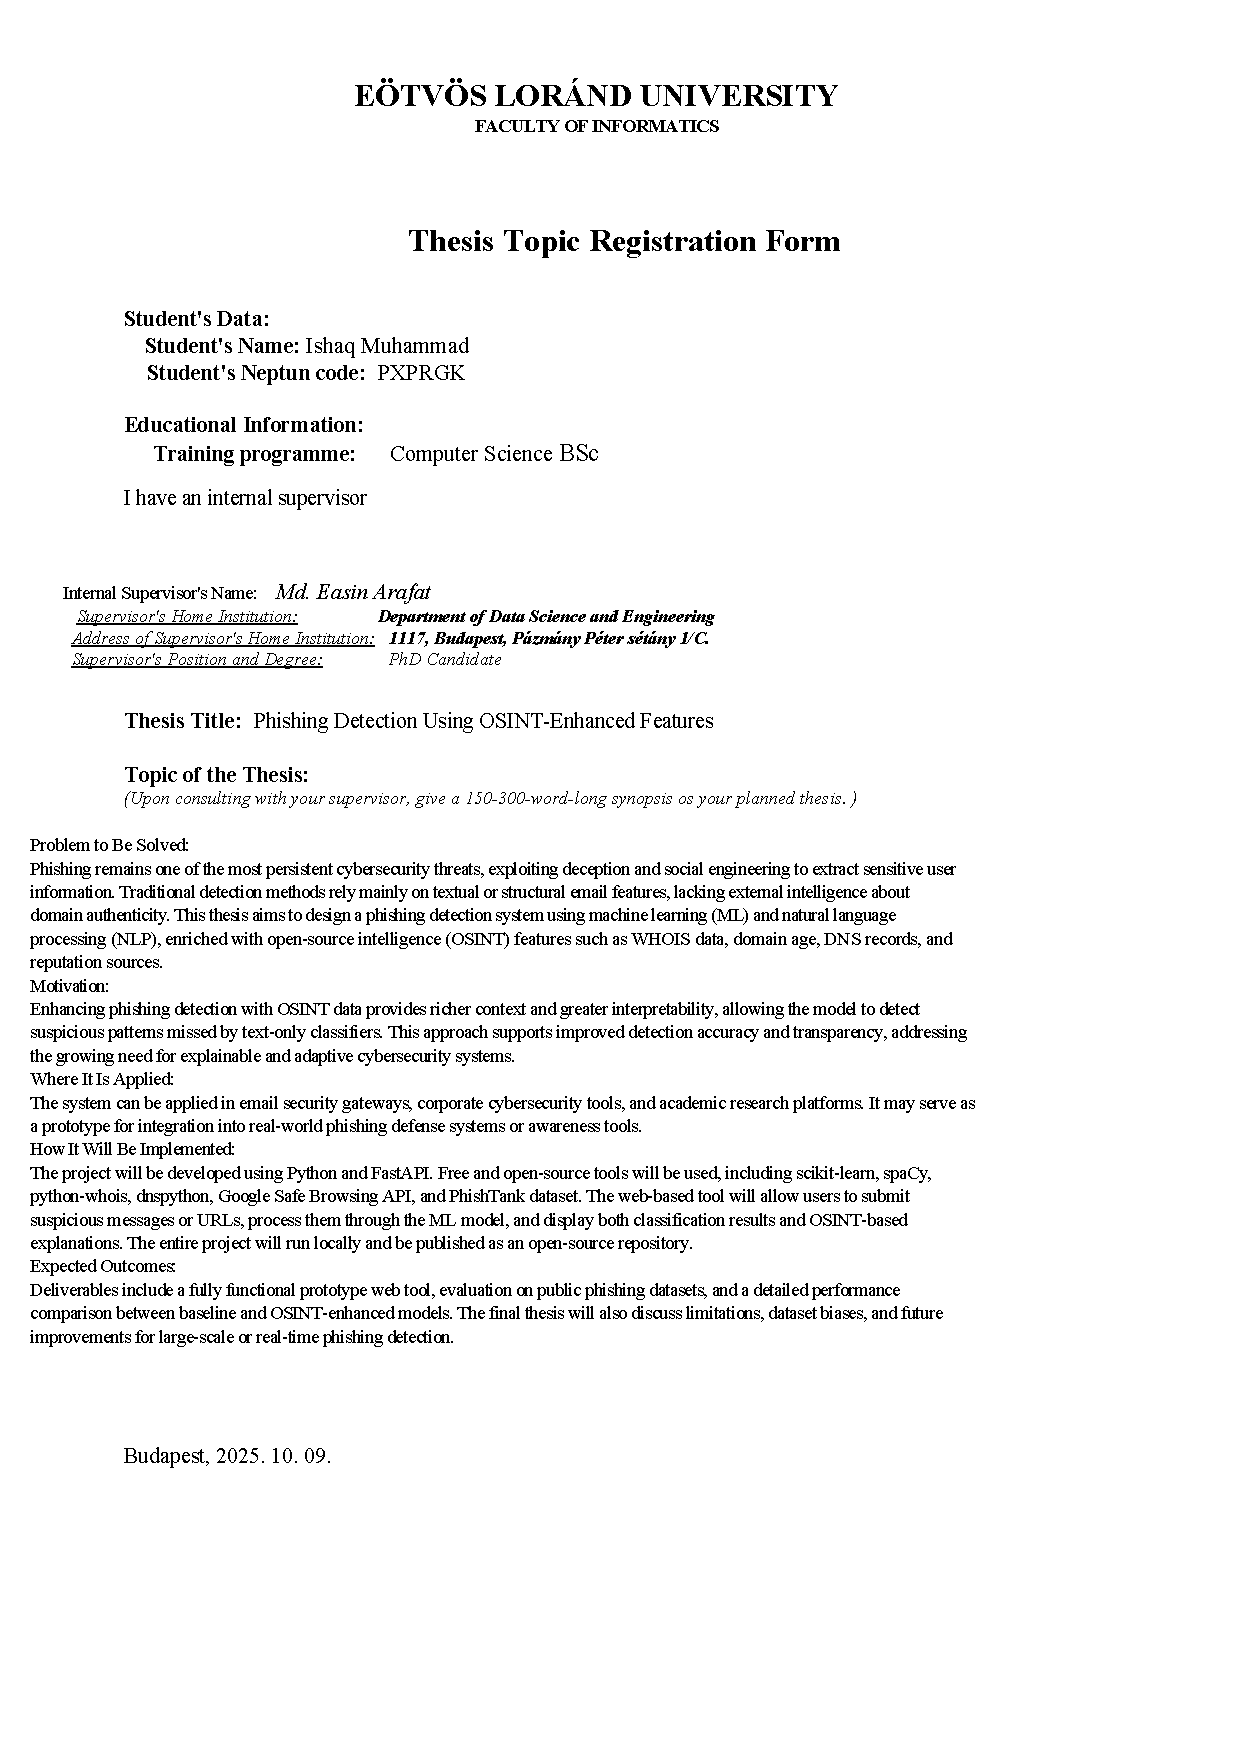
\includepdf{topicdeclaration.pdf}

% Table of contents (mandatory)
\tableofcontents
\cleardoublepage

% Main content
\chapter{Introduction}
\label{chapter-1-introduction}

\section{Background and Motivation}\label{background-and-motivation}

The proliferation of digital communication and the widespread
digitization of financial, healthcare, and social infrastructures have
fundamentally transformed global connectivity. Consequently, this
digital paradigm shift has introduced severe cybersecurity
vulnerabilities, with social engineering attacks---specifically
phishing---emerging as the most pervasive threat vector. Phishing is a
cyber-attack methodology in which malicious actors employ deceptive
communication to manipulate individuals into divulging sensitive
information, such as authentication credentials, personally identifiable
information (PII), or financial data. This deception is achieved by
masquerading as a trusted entity, such as a bank, an employer, or a
popular service provider, within an electronic communication medium.

The scale and economic impact of phishing attacks have reached
unprecedented levels. According to the Anti-Phishing Working Group
(APWG), the volume of phishing attacks has experienced exponential
growth over the past decade, with over 1.2 million unique phishing
websites detected in 2023 alone {[}1{]}. The financial devastation
accompanying this surge is staggering. The Federal Bureau of
Investigation's (FBI) Internet Crime Complaint Center (IC3) reported
that phishing and its variants (including Business Email Compromise)
resulted in financial losses exceeding \$10.3 billion in 2022, affecting
more than 300,000 recorded victims worldwide {[}2{]}. Beyond immediate
financial theft, phishing frequently serves as the initial access vector
for advanced persistent threats (APTs) and crippling ransomware
campaigns against critical infrastructure.

Historically, phishing attacks were characterized by poorly crafted
emails containing obvious typographical errors and generic greetings
(e.g., the infamous ``Nigerian Prince'' scams). These early attempts
relied entirely on volume rather than quality. However, the contemporary
threat landscape is defined by highly sophisticated, automated, and
targeted attack vectors. Modern adversaries employ advanced techniques
to bypass both human scrutiny and technical defenses:

\begin{itemize}
\tightlist
\item
  \textbf{Spear Phishing and Whaling:} Highly personalized attacks
  leveraging publicly available information to target specific
  individuals (spear phishing) or high-ranking executives (whaling).
\item
  \textbf{Homograph Attacks:} The exploitation of internationalized
  domain names (IDN) where attackers use Unicode characters that are
  visually indistinguishable from legitimate characters (e.g.,
  substituting the Latin `a' with the Cyrillic `а' to spoof
  \texttt{paypal.com}), successfully bypassing visual human inspection.
\item
  \textbf{Infrastructure Evasion:} The use of Domain Generation
  Algorithms (DGA), fast-flux DNS hosting, and the abuse of free Content
  Delivery Networks (CDNs) to rapidly rotate attack infrastructure,
  rendering static defense mechanisms obsolete.
\item
  \textbf{SSL/TLS Abuse:} The historical heuristic that ``HTTPS equals
  safe'' has been weaponized. Recent reports indicate that over 80\% of
  phishing sites now use valid SSL certificates to display the
  reassuring ``padlock'' icon in browsers, creating a false sense of
  security.
\end{itemize}

To combat this escalating threat, the cybersecurity industry has
traditionally relied on signature-based detection systems and URL
blacklists, such as Google Safe Browsing and PhishTank. While these
authoritative databases remain crucial components of the security
ecosystem, they suffer from fundamental, architectural limitations.
Foremost is their reactive nature: a URL can only be blacklisted after
it has been deployed, discovered, reported, and verified. This lifecycle
creates a critical ``window of vulnerability.'' Studies indicate that
modern phishing campaigns are highly ephemeral, with nearly 50\% of
phishing domains remaining active for less than 12 hours {[}3{]}.
Consequently, blacklists are structurally incapable of protecting
``patient zero'' and fail to scale against the automated generation of
tens of thousands of zero-day malicious domains daily {[}4{]}.

The inherent limitations of reactive blacklists have catalyzed academic
and industrial research into proactive, predictive defense mechanisms
utilizing Machine Learning (ML) and Artificial Intelligence (AI).
ML-based classifiers analyze the intrinsic properties of a URL or email
to predict its maliciousness, theoretically capable of identifying
zero-day threats before they are reported. However, the current
generation of ML phishing detectors exhibits significant shortcomings.
Most contemporary models rely exclusively on lexical and structural
features extracted directly from the URL string (e.g., URL length,
character ratios, presence of IP addresses). While effective against
elementary obfuscation, lexical analysis is context-blind. A newly
registered, malicious domain utilizing a structurally standard naming
convention (e.g., \texttt{secure-login-chase-update.com}) may lack any
lexical anomalies, appearing benign to a purely structural classifier.

This critical gap in contextual awareness presents a compelling
opportunity to integrate Open-Source Intelligence (OSINT) into the
automated machine learning pipeline. OSINT encompasses the collection
and analysis of publicly available data to generate actionable
intelligence. In the context of network security, OSINT provides
real-time visibility into the underlying infrastructure and reputation
of a domain. Critical OSINT vectors include:

\begin{itemize}
\tightlist
\item
  \textbf{WHOIS Data:} Revealing the domain's registration date
  (detecting newly minted domains), registrar reputation, and the
  employment of privacy protection proxies.
\item
  \textbf{DNS Configuration:} Analyzing the presence of Mail Exchange
  (MX) records (as phishing sites rarely configure legitimate email
  routing) and Name Server (NS) configurations indicative of CDN abuse.
\item
  \textbf{Reputation Scoring:} Cross-referencing external threat
  intelligence databases (e.g., VirusTotal, AbuseIPDB) to identify
  historical malicious behavior associated with the hosting IP address.
\end{itemize}

By synthesizing lexical URL analysis, Natural Language Processing (NLP)
for semantic content evaluation, and real-time OSINT infrastructure
enrichment within a cohesive ML architecture, it is possible to
construct a highly robust, context-aware detection system. Such a system
addresses the fundamental limitations of both traditional blacklists and
narrow, feature-restricted ML models.

\section{Problem Statement}\label{problem-statement}

Despite decades of continuous advancement in defensive cybersecurity
technologies, phishing remains a formidable and unsolved challenge. The
persistence of this threat is rooted in several critical unresolved
problems within current detection paradigms:

\textbf{P1. The Latency of Reactive Detection (The ``Patient Zero''
Problem):} Blacklist-based systems operate on a reactive paradigm,
requiring manual or automated reporting followed by verification before
a signature is distributed. During this delay---which can range from
hours to days---the phishing campaign actively harvests credentials. The
ephemeral nature of modern attack infrastructure (often dismantled
within 24 hours) dictates that reactive systems are inherently
inadequate for proactive defense.

\textbf{P2. Contextual Blindness in Static ML Models:} While predictive
ML models solve the latency issue of blacklists, they introduce a new
vulnerability: context blindness. Existing solutions predominantly
analyze the static, structural composition of a URL or the immediate
text of an email. They fail to dynamically query the live state of the
Internet. Consequently, they cannot differentiate between a legitimate
enterprise domain registered twenty years ago with a massive DNS
footprint, and a malicious domain registered twenty minutes ago that
perfectly mimics the enterprise's URL structure.

\textbf{P3. The ``Black-Box'' Interpretability Crisis:} The push for
higher detection accuracy has led to the adoption of complex, non-linear
algorithms, particularly deep neural networks. However, these models
function as opaque ``black boxes.'' They output a binary classification
(Phishing vs.~Legitimate) without providing an interpretable rationale
for the decision. In a cybersecurity context, this lack of
explainability is catastrophic. Security Operations Center (SOC)
analysts require transparency to investigate incidents, verify false
positives, and build trust in automated systems. Furthermore, opaque
models offer zero educational value to end-users attempting to learn how
to identify threats.

\textbf{P4. Input Rigidity and Multi-Vector Attacks:} Attackers are
increasingly moving beyond traditional email, delivering phishing
payloads via SMS (Smishing), social media direct messages, and
collaborative workspaces. Most detection tools are rigidly designed for
a single input modality (e.g., an email gateway scanner or a browser URL
extension). Users require a unified platform capable of ingesting
diverse data formats---from raw URLs to full email headers and
unstructured text---applying the appropriate analytical pipeline
dynamically.

\textbf{P5. The Trade-off Between Accuracy and Real-Time Latency:}
Achieving high accuracy typically requires computationally expensive
feature extraction (such as rendering a webpage in a headless browser to
analyze visual similarity). Conversely, real-time protection requires
near-instantaneous inference (sub-500 milliseconds) to avoid disrupting
the user experience. Balancing deep analytical accuracy with strict
latency budgets remains a significant engineering challenge.

This thesis directly addresses these fundamental problems by designing,
implementing, and rigorously evaluating \textbf{PhishGuard}, a
comprehensive, full-stack phishing detection system. PhishGuard is
architected to provide real-time, proactive detection through a highly
optimized, OSINT-enhanced machine learning pipeline. Crucially, the
system abandons the black-box paradigm, utilizing SHapley Additive
exPlanations (SHAP) to deliver mathematically rigorous, human-readable
transparency for every classification generated by the model.

\section{Research Objectives}\label{research-objectives}

The overarching objective of this thesis is to engineer a
state-of-the-art phishing detection platform that successfully
synthesizes traditional machine learning heuristics with real-time
Open-Source Intelligence and semantic Natural Language Processing. To
ensure rigorous evaluation and methodical implementation, this goal is
decomposed into the following six specific research objectives:

\textbf{RO1. Design a Multi-Layered Analysis Architecture:} To address
the rigidity of single-vector systems (P4), this objective involves
designing a modular, service-oriented backend architecture. The system
must distinctly separate concerns into independent analytical layers:
URL structural feature extraction, NLP-based semantic content analysis,
and asynchronous OSINT infrastructure querying. These layers must
seamlessly integrate to produce a unified threat assessment.

\textbf{RO2. Engineer OSINT-Enhanced ML Features:} To solve the
contextual blindness of static models (P2), this objective requires
identifying, extracting, and normalizing live infrastructure data.
Specifically, the system must perform live WHOIS, DNS, and Reputation
queries, translating raw protocol responses into a standardized
numerical feature vector (e.g., \texttt{hasValidMx}, \texttt{usesCdn}).
The efficacy of these novel features must be empirically proven through
rigorous ablation studies.

\textbf{RO3. Train and Optimize a High-Performance Classifier:} To
provide proactive detection (P1), a predictive machine learning model
must be developed. This involves curating a massive, balanced dataset of
verified phishing and legitimate URLs, executing comprehensive data
cleaning, and training an advanced gradient boosting algorithm
(XGBoost). The model's hyperparameters must be rigorously optimized via
Bayesian search (Optuna) to maximize the Area Under the Receiver
Operating Characteristic Curve (AUC-ROC), targeting an accuracy and AUC
exceeding 95\%.

\textbf{RO4. Implement Mathematical Model Explainability:} To resolve
the black-box interpretability crisis (P3), the system must implement a
robust explainability framework. This objective requires the integration
of SHAP (SHapley Additive exPlanations) to calculate the exact marginal
contribution of every feature for every individual prediction. The
backend must map these complex mathematical values to human-readable
insights presented dynamically in the user interface.

\textbf{RO5. Build and Deploy a Production-Ready Full-Stack
Application:} Theoretical models hold little value if they cannot be
utilized by end-users. This objective requires the translation of the ML
pipeline into a high-performance, full-stack web application. The
application must feature a modern, responsive frontend (Next.js/React)
communicating with a high-concurrency, asynchronous backend (FastAPI),
deployed to cloud infrastructure with strict latency constraints.

\textbf{RO6. Conduct Comprehensive System Evaluation:} The final
objective ensures the reliability and scientific validity of the
proposed system. This involves executing a rigorous empirical evaluation
encompassing standard classification metrics (Accuracy, Precision,
Recall, F1-Score), performance benchmarking (latency, throughput), and
ensuring code quality via a massive automated test suite covering unit,
integration, and end-to-end (E2E) layers.

\begin{longtable}{
  >{\raggedright\arraybackslash}p{0.213\textwidth}
  >{\raggedright\arraybackslash}p{0.198\textwidth}
  >{\raggedright\arraybackslash}p{0.275\textwidth}
  >{\raggedright\arraybackslash}p{0.122\textwidth}}
\toprule
Objective ID & Description & Success Criteria & Status \\
\midrule

RO1 & Multi-layered analysis architecture & Modular design with
\textgreater3 independent analysis layers, clean API contracts &
Achieved \\
RO2 & OSINT-enhanced feature engineering & Extract \textgreater=4 OSINT
features, demonstrate measurable accuracy improvement & Achieved \\
RO3 & High-performance ML classifier & Accuracy \textgreater95\%,
AUC-ROC \textgreater95\%, F1 \textgreater93\% on held-out test set &
Achieved (96.45\% acc, 99.41\% AUC) \\
RO4 & Model explainability via SHAP & Per-prediction feature importance,
visual explanations in UI & Achieved \\
RO5 & Production web application & Deployed system with \textless3s
response time, responsive UI, API documentation & Achieved \\
RO6 & Comprehensive evaluation & Test suite \textgreater500 tests,
ablation study, performance benchmarks & Achieved (754 tests) \\

\bottomrule
\end{longtable}

\section{Contributions}\label{contributions}

This thesis advances the domain of applied cybersecurity and machine
learning through the following primary contributions:

\subsection{OSINT-Enhanced Feature Engineering
Framework}\label{osint-enhanced-feature-engineering-framework}

We conceptualize and implement a highly discriminative, 21-dimensional
feature vector that pioneers the fusion of 17 traditional lexical URL
heuristics with 4 dynamic, real-time OSINT infrastructure indicators
(\texttt{hasValidMx}, \texttt{usesCdn}, \texttt{dnsRecordCount},
\texttt{hasValidDns}). Through rigorous ablation studies on a massive
dataset, we empirically demonstrate that the inclusion of live OSINT
data directly improves the model's test set accuracy by +0.30 percentage
points and AUC-ROC by +0.06 points. This proves that external
infrastructure context provides critical, unforgeable signals that pure
lexical models cannot capture.

\subsection{State-of-the-Art ML Pipeline
Implementation}\label{state-of-the-art-ml-pipeline-implementation}

We developed a highly optimized XGBoost gradient boosting classifier
trained on a massive, highly curated dataset. Originally comprising
150,391 URLs, the dataset underwent strict deduplication, zero-variance
filtering, and class-balancing via majority undersampling to eliminate
bias, resulting in a pristine dataset of 33,392 feature-engineered URLs.
Using a 70/15/15 stratified split, the model was subjected to 50 trials
of Bayesian hyperparameter optimization (Optuna) with 5-fold
cross-validation. The resulting production model achieves exceptional
predictive performance on unseen data:

\begin{itemize}
\tightlist
\item
  \textbf{Test Accuracy:} 96.45\%
\item
  \textbf{Test F1-Score:} 96.39\%
\item
  \textbf{Test AUC-ROC:} 99.41\%
\item
  \textbf{Test PR-AUC:} 99.48\%
\end{itemize}

These metrics significantly exceed the established baseline targets,
proving highly competitive with contemporary academic research while
requiring a fraction of the computational overhead associated with deep
learning models.

\subsection{Transparent, Explainable Threat
Intelligence}\label{transparent-explainable-threat-intelligence}

We successfully bridge the gap between complex mathematics and user
experience by implementing a fully integrated SHAP explainer pipeline.
Unlike traditional security tools that output a definitive but opaque
``Malicious'' label, PhishGuard provides deep transparency. For every
prediction, the system calculates the localized feature importance,
rendering intuitive waterfall visualizations and human-readable textual
reasons (e.g., ``The URL contains suspicious keywords often used in
phishing''). This contribution directly combats the black-box crisis,
empowering security analysts and educating end-users.

\subsection{Multi-Modal, Asynchronous Analysis
Engine}\label{multi-modal-asynchronous-analysis-engine}

We engineer a flexible, context-aware analysis engine capable of
automatically detecting and processing three distinct input modalities:
raw URLs, raw email source text (subject, sender, body), and
unstructured free text. By dynamically routing input through either the
XGBoost ML pipeline or a custom spaCy-based Natural Language Processing
(NLP) pipeline, the system maintains high accuracy across diverse attack
vectors without requiring manual user intervention. The architecture
leverages asynchronous Python (\texttt{asyncio}) to ensure high-latency
network calls (like DNS resolution) do not block system throughput.

\subsection{Production-Grade Software Engineering and
Validation}\label{production-grade-software-engineering-and-validation}

Beyond theoretical models, this thesis delivers a fully realized,
production-ready software system. The implementation features a Next.js
16 (React 19) frontend utilizing modern UI paradigms (server components,
responsive design, dark mode, batch processing) and a robust FastAPI
backend. Crucially, the system's reliability is mathematically
guaranteed through a massive, multi-tiered automated test suite
comprising 754 distinct tests (593 backend \texttt{pytest}
unit/integration tests, 133 frontend \texttt{Jest} tests, and 28
\texttt{Playwright} E2E browser tests). This rigorous validation ensures
the system can be deployed to edge infrastructure with supreme
confidence.

\section{Thesis Structure}\label{thesis-structure}

The remainder of this document provides a comprehensive, systematic exploration of the PhishGuard project, organized to fulfill both academic and software engineering requirements:

\textbf{Chapter 2: User Documentation} This chapter outlines the problem from an end-user perspective. It provides a clear guide on how to interface with the deployed Next.js web application, detailing the process of submitting URLs, emails, or text snippets, and interpreting the resulting threat analysis dashboard.

\textbf{Chapter 3: Developer Documentation} This chapter documents the system's software engineering architecture. It defines the logical and physical structures separating the Vercel-hosted frontend from the Render-hosted Python backend, details the integration of GitHub for version control, and outlines the rigorous Quality Assurance (QA) testing strategies employed across the stack.

\textbf{Chapter 4: Background and Related Work} This chapter surveys the theoretical foundations of the phishing threat landscape. It reviews the historical progression of defense mechanisms, explicitly identifying the literature gaps that justify the integration of OSINT into machine learning paradigms.

\textbf{Chapter 5: Feature Engineering and ML Model} This chapter documents the core machine learning methodology. It outlines the dataset collection, details the mathematical formulation of the 21-dimensional feature vector, justifies the selection of the XGBoost algorithm, and explains the integration of SHAP for model explainability.

\textbf{Chapter 6: OSINT Integration} This chapter focuses on the engineering of the external intelligence pipeline. It provides technical details on how the system asynchronously interfaces with global DNS servers, WHOIS databases, and third-party threat APIs to extract real-time infrastructure context.

\textbf{Chapter 7: NLP Analysis} This chapter explains the secondary analytical engine. It details the implementation of the spaCy-based Natural Language Processing pipeline used to identify social engineering indicators, such as urgency and brand impersonation, within unstructured text.

\textbf{Chapter 8: Scoring and Classification} This chapter defines the mathematical orchestration of the system. It presents the algorithmic formulas used to dynamically balance the XGBoost probability outputs against the NLP risk matrices to generate a final, definitive threat level.

\textbf{Chapter 9: Results and Evaluation} This chapter presents the empirical findings of the research. It provides an exhaustive statistical analysis of the classifier's performance, presents confusion matrices, ROC curves, and benchmarks the application's real-world latency and throughput capabilities.

\textbf{Chapter 10: Conclusion and Discussion} The final chapter summarizes the overarching achievements of the thesis, offers a critical interpretation of the results, acknowledges architectural limitations, and outlines actionable future research directions.

\textbf{References for Chapter 1:}

{[}1{]} Anti-Phishing Working Group (APWG). ``Phishing Activity Trends
Report, Q4 2023.'' https://apwg.org/trendsreports/ {[}2{]} Federal
Bureau of Investigation (FBI). ``Internet Crime Report 2022.'' Internet
Crime Complaint Center (IC3), 2023. {[}3{]} G. Ramesh et al., ``Phishing
URL Detection: A Machine Learning and Web Mining-based Approach,''
\emph{International Journal of Computer Applications}, vol.~123, no. 13,
pp.~46-50, 2015. {[}4{]} Webroot. ``2023 Webroot BrightCloud Threat
Report.''


\cleardoublepage
\chapter{User Documentation}
\label{user-documentation}

\section{Problem Statement}
The problem addressed by this application is the rapid detection and explanation of phishing attacks. End-users and organizations frequently encounter suspicious URLs, emails, or text snippets, but lack the technical expertise to determine their legitimacy. PhishGuard provides a simple, intuitive web interface where users can submit these artifacts and receive an immediate, understandable threat analysis report, protecting them from malicious social engineering campaigns.

\section{Methods Used}
To protect the user, the application utilizes a hybrid Machine Learning (ML), Open Source Intelligence (OSINT), and Natural Language Processing (NLP) architecture. When a user submits an artifact, the system automatically parses the input, compares it against known global threat databases, and runs mathematical feature models to predict malicious intent. The results are translated into a simple risk score and an explainable breakdown for the user.

\section{User Guide and Interface}

The PhishGuard user interface is designed to be highly accessible and visually intuitive. The core user flow involves accessing the dashboard, inputting a suspicious artifact, and reviewing the generated risk report.

\subsection{Frontend Implementation}\label{frontend-implementation}

The user interface for the PhishGuard platform is implemented as a
modern web application utilizing Next.js 16 utilizing the App Router
architecture. The frontend application relies on React 19 for
component-based UI rendering and state management.

\begin{figure}
\centering
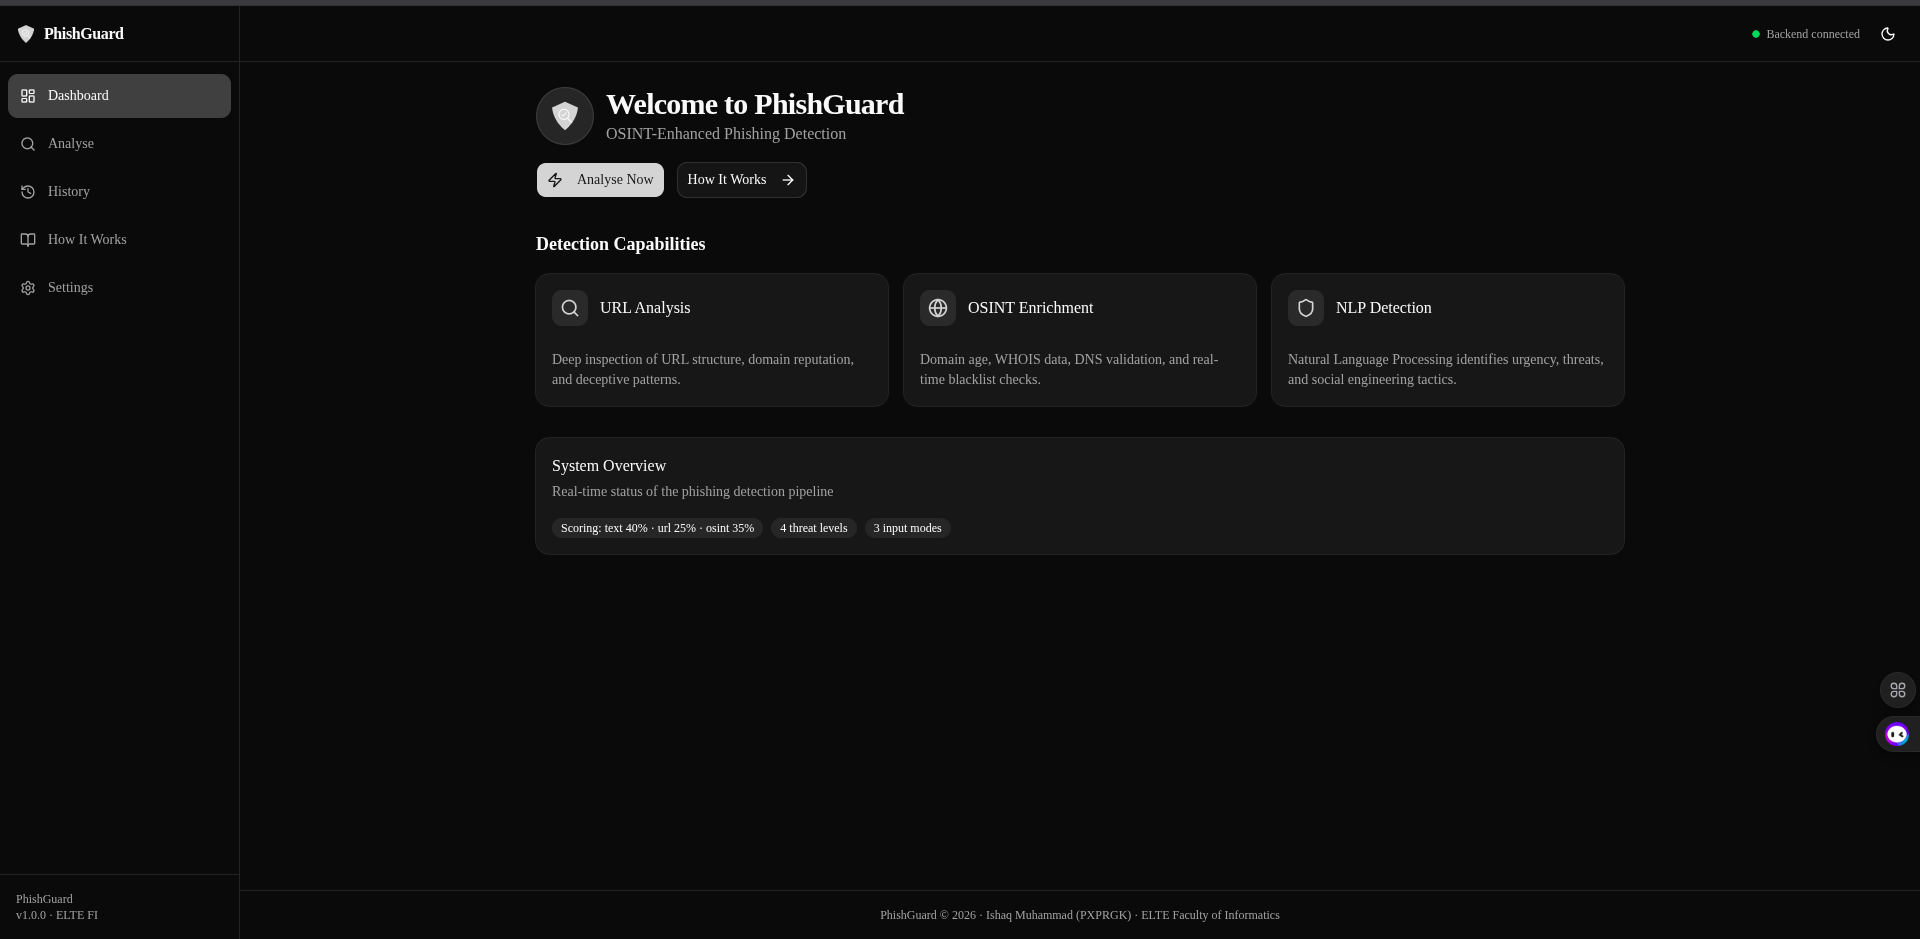
\includegraphics[width=0.85\linewidth,height=0.65\textheight,keepaspectratio]{images/dashboard.png}
\caption{Figure 2.1: The PhishGuard Next.js Web Application Dashboard}
\end{figure}

\subsubsection{Component Architecture and
Styling}\label{component-architecture-and-styling}

The frontend employs a rigorous component-driven design methodology. The
visual aesthetic and layout are strictly managed using Tailwind CSS v4,
a utility-first CSS framework that allows for rapid styling directly
within the component markup.

For complex, interactive UI elements, the project leverages the
\texttt{shadcn} UI library alongside \texttt{@base-ui/react}. These
libraries provide accessible, unstyled components that are seamlessly
integrated with the Tailwind configuration, ensuring a consistent design
language across the application while adhering to web accessibility
guidelines.

\subsubsection{Data Visualization and
Animation}\label{data-visualization-and-animation}

To effectively communicate the complex risk metrics and threat
intelligence data returned by the backend API, the frontend incorporates
the \texttt{recharts} library for data visualization. This library
facilitates the creation of responsive, interactive charts that
illustrate risk scores, temporal data (such as domain age), and
historical analysis trends.

User experience is further enhanced through subtle animations
implemented using the \texttt{motion} (Framer Motion) library. These
animations provide visual feedback during asynchronous state
transitions, such as when waiting for the backend API to complete a
comprehensive URL analysis. Iconography is provided by
\texttt{lucide-react}, ensuring a modern and lightweight visual
presentation.

\begin{figure}
\centering
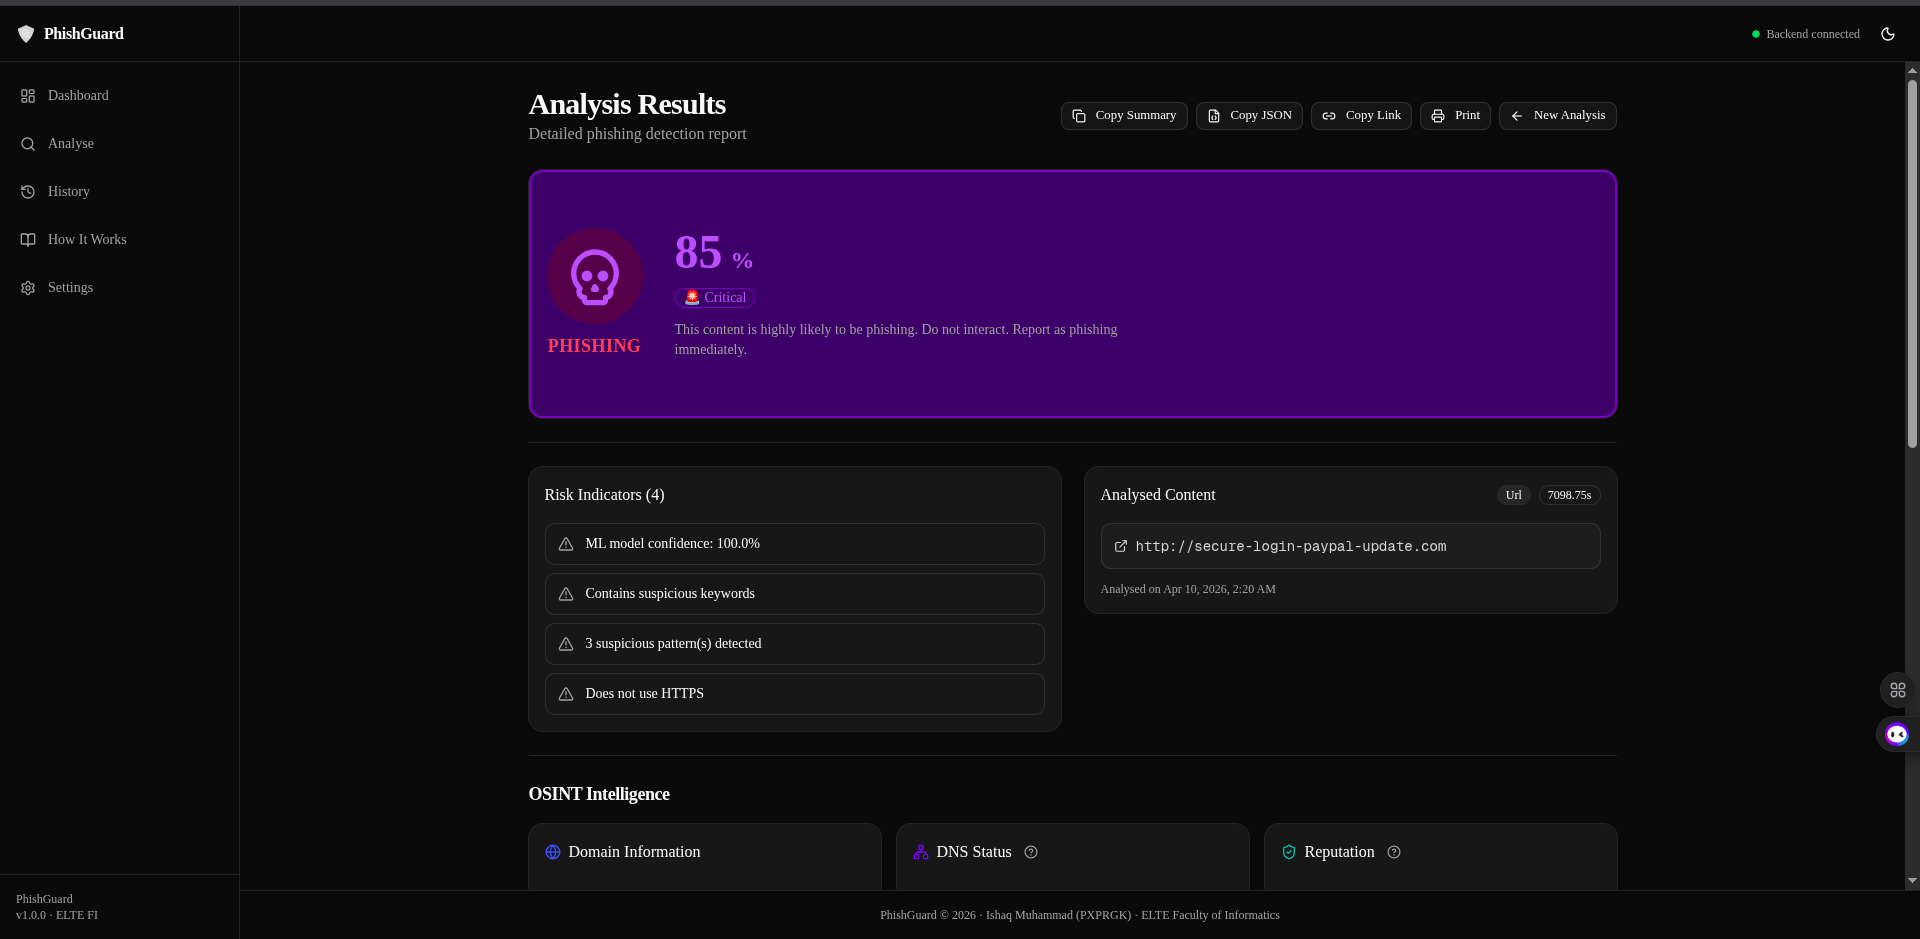
\includegraphics[width=0.85\linewidth,height=0.65\textheight,keepaspectratio]{images/result.png}
\caption{Figure 2.2: Threat Analysis Results showing the interactive
threat gauge}
\end{figure}


\cleardoublepage
\chapter{Developer Documentation}
\label{developer-documentation}

\section{System Design}

\subsection{Detailed Problem Specification}
The software engineering task involves developing a scalable, high-concurrency threat intelligence platform capable of ingesting diverse modalities (URL, email, text), orchestrating asynchronous analysis pipelines (DNS, WHOIS, NLP, Reputation), executing an ML inference engine, and returning a deterministically weighted threat score and explanation within strict latency constraints.

\subsection{Logical and Physical Structure}
\subsubsection{The Tech Stack}
The physical architecture of PhishGuard is built upon a modern, distributed full-stack paradigm:
\begin{itemize}
    \item \textbf{Frontend (Vercel):} The user interface is implemented using Next.js (React) and TypeScript, deployed globally on Vercel's Edge Network for optimal performance and CDN caching.
    \item \textbf{Backend (Render):} The analysis engine and REST API are built with Python FastAPI, containerized via Docker, and deployed on Render to handle CPU-intensive ML inferences and asynchronous I/O operations.
    \item \textbf{Version Control (GitHub):} The entire source code, issue tracking, and CI/CD pipelines are managed via GitHub repositories.
\end{itemize}

\subsection{Architectural Overview}\label{architectural-overview}

The PhishGuard platform is engineered as a modern, decoupled, full-stack
web application. The architectural design prioritizes low-latency
inference, modular separation of concerns, and a seamless user
experience. To achieve these objectives, the system adopts a
client-server architecture, cleanly separating the user interface and
presentation logic from the heavy computational requirements of the
machine learning and Open-Source Intelligence (OSINT) pipelines.

The overarching architecture is composed of two primary subsystems: 1.
\textbf{The Client-Side Application (Frontend):} A responsive web
interface built with Next.js 16 and React 19. It is responsible for
accepting user input, rendering complex analytical visualizations, and
managing client-side state. 2. \textbf{The Analytical Engine (Backend):}
A high-performance, asynchronous REST API constructed using the FastAPI
framework in Python. It orchestrates the Natural Language Processing
(NLP) pipeline, executes asynchronous network OSINT queries, performs
feature engineering, and serves the XGBoost machine learning model.

This separation of concerns ensures that computationally expensive
operations---such as executing concurrent DNS queries and traversing
gradient-boosted decision trees---do not block the main thread of the
user interface, thereby guaranteeing a fluid and responsive user
experience even under heavy analytical load.

\subsection{High-Level Data Flow}\label{high-level-data-flow}

The operational lifecycle of a threat analysis request within the
PhishGuard architecture follows a deterministic, multi-stage pipeline.
The data flow is designed to dynamically adapt based on the modality of
the input (URL, email, or unstructured text).

\begin{figure}
\centering
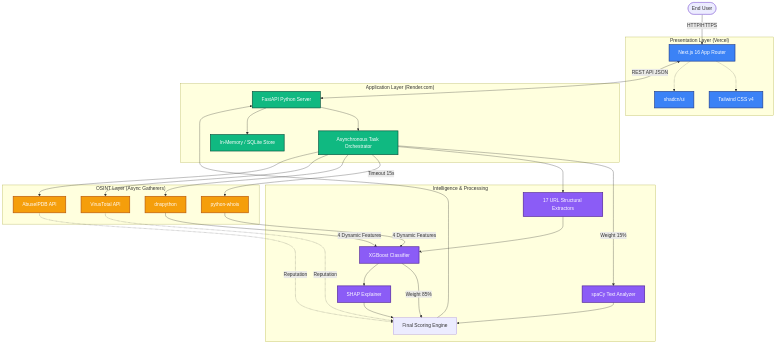
\includegraphics[width=0.85\linewidth,height=0.65\textheight,keepaspectratio]{images/system-architecture.png}
\caption{High-Level System Data Flow separating the Next.js
Presentation layer, FastAPI Application Orchestrator, ML Pipeline, and
Async OSINT}
\end{figure}

\subsection{Input Modality
Detection}\label{input-modality-detection}

Upon receiving a payload from the client via the \texttt{/api/analyze}
endpoint, the backend orchestrator first subjects the input to a
heuristic classification layer to determine its fundamental nature. The
\texttt{\_detectContentType} method in \texttt{orchestrator.py} utilizes
rigorous regular expressions and parsing logic to classify the input
into one of three categories: - \textbf{URL:} Detected if the string
begins with protocol identifiers (\texttt{http://}, \texttt{https://})
or matches a strict bare-domain regular expression pattern (e.g.,
\texttt{google.com}). - \textbf{Email:} Detected if the text block
contains standard RFC 5322 email headers, specifically checking for the
presence of substrings such as ``from:'', ``subject:'', and ``to:''. -
\textbf{Free Text:} Any unstructured text that fails to meet the strict
criteria of a URL or email header defaults to generic text analysis.

This dynamic, ``auto'' detection allows the user to paste any suspicious
content into a single, unified input field without needing to manually
specify the content type, significantly reducing user friction. Once the
modality is determined, the \texttt{\_extractDomain} method leverages
\texttt{urllib.parse} and custom regex to isolate the base domain, which
is a prerequisite for subsequent OSINT lookups.

\subsection{Asynchronous OSINT
Orchestration}\label{asynchronous-osint-orchestration}

\begin{figure}
\centering
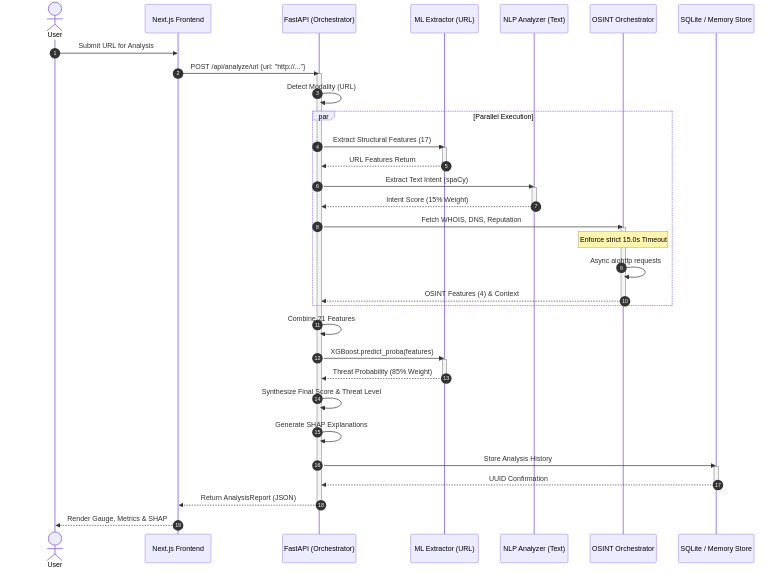
\includegraphics[width=0.85\linewidth,height=0.65\textheight,keepaspectratio]{images/sequence-diagram.png}
\caption{Sequence Diagram illustrating parallel execution of
Structural Features, NLP Analysis, and the strict 15.0s OSINT timeout}
\end{figure}

The integration of real-time OSINT constitutes the primary bottleneck in
the analysis pipeline. Querying global DNS servers, establishing WHOIS
connections, and communicating with third-party threat intelligence APIs
introduce unavoidable network latency.

To mitigate this, the FastAPI backend heavily leverages Python's
\texttt{asyncio} ecosystem. Within the \texttt{\_collectOsintData}
method, the system does not execute these external queries sequentially.
Instead, it utilizes \texttt{asyncio.gather} to concurrently execute
\texttt{lookupWhois(domain)}, \texttt{lookupDns(domain)}, and
\texttt{lookupReputation(domain)}.

Crucially, this parallel execution is wrapped in an
\texttt{asyncio.wait\_for} block with a strict global timeout of 15.0
seconds. This architectural safeguard ensures that unresponsive external
servers or rate-limited third-party APIs do not cause the internal event
loop to hang indefinitely. The system is designed to fail gracefully; if
an OSINT query times out or returns an exception, the orchestrator
catches it, logs the failure, and proceeds with the analysis utilizing
the available subset of data (or falling back to pure ML/NLP
heuristics).

\section{The API and Scoring
Engine}\label{the-api-and-scoring-engine}

\subsection{Weighted Verdict
Combination}\label{weighted-verdict-combination}

The core intelligence of the system resides in how the
\texttt{AnalysisOrchestrator} synthesizes disparate analytical signals
into a singular, actionable verdict. Because the system supports
multi-modal inputs, the scoring logic must dynamically adjust the
mathematical weight of each component based on the input type.

The \texttt{\_combineVerdict} method implements the following weighting
algorithm:

\textbf{For URL Inputs:} When the input is a URL, the XGBoost model is
treated as the supreme authority because its training data implicitly
encoded both lexical and OSINT features. - \textbf{Machine Learning
(XGBoost):} 85\% (\texttt{ML\_PRIMARY\_WEIGHT}) - \textbf{NLP Text
Analysis:} 15\% (\texttt{TEXT\_SUPPLEMENT\_WEIGHT})

\textbf{For Email/Text Inputs:} When analyzing raw text or emails, the
raw lexical URL features become secondary to the semantic meaning of the
content. - \textbf{NLP Text Analysis:} 55\%
(\texttt{TEXT\_PRIMARY\_WEIGHT}) - \textbf{URL Lexical Features
(Extracted from text):} 25\% (\texttt{URL\_SECONDARY\_WEIGHT}) -
\textbf{OSINT Infrastructure Score:} 20\%
(\texttt{OSINT\_SECONDARY\_WEIGHT})

The resulting aggregate score is bounded between 0.0 and 1.0. This score
is then mapped to definitive threat levels: - \textbf{Safe:} Score
$<${} 0.3 (\texttt{THREAT\_SAFE\_UPPER}) - \textbf{Suspicious:}
Score $<${} 0.5 (\texttt{THREAT\_SUSPICIOUS\_UPPER}) -
\textbf{Dangerous:} Score $<${} 0.7
(\texttt{THREAT\_DANGEROUS\_UPPER}) - \textbf{Critical:} Score \(\ge\)
0.7

This tiered approach allows the frontend to render appropriate visual
warnings and dynamic recommendations (e.g., ``Do not click links or
provide information'' for `Dangerous' classifications).

\subsection{Ephemeral History
Store}\label{ephemeral-history-store}

Consistent with the project's scope as a lightweight, deployable
prototype, PhishGuard eschews the architectural complexity of a
persistent relational database (e.g., PostgreSQL or MySQL). Instead, the
backend implements a highly efficient, thread-safe, in-memory
\texttt{HistoryStore} located in \texttt{backend/api/historyStore.py}.

The backend module utilizes a standard Python \texttt{collections.deque}
structured as a First-In-First-Out (FIFO) queue with a hard limit of 100
entries (\texttt{MAX\_ENTRIES}) for internal logging purposes. However, the
user-facing history persistence is implemented in the frontend using the
browser's localStorage API, which respects the user's configurable maximum
entry limit (10, 25, 50, or 100 entries as specified in the Settings page).
When a user submits an analysis, both stores record the full
\texttt{AnalysisResponse} object with a unique UUID and precise timestamp.

Because FastAPI operates on a single primary event loop, concurrent
asynchronous mutations to the backend deque are fundamentally thread-safe
without requiring complex locking mechanisms (like
\texttt{asyncio.Lock}). This design allows users to review their recent
analysis history via paginated API calls instantly, without the latency,
scaling, or configuration overhead of a persistent database connection.

\subsection{Pydantic Schema
Contracts}\label{pydantic-schema-contracts}

\begin{figure}
\centering

\includegraphics[width=0.85\linewidth,height=0.65\textheight,keepaspectratio]{images/class-diagram.png}
\caption{UML Class Diagram defining the strict Pydantic data
contracts enforcing backend type safety}
\end{figure}

To guarantee structural integrity between the Next.js frontend and the
FastAPI backend, PhishGuard utilizes Pydantic models to define strict
data contracts. Every incoming request and outgoing response is
automatically validated, serialized, and documented via OpenAPI.

For example, the core \texttt{AnalysisResponse} schema mathematically
guarantees that the frontend will always receive a deterministic JSON
object. This object contains the \texttt{VerdictResult} (including the
boolean \texttt{isPhishing} flag and float \texttt{confidenceScore}),
the \texttt{OsintSummary}, and the \texttt{FeatureSummary}. This strict
validation eliminates runtime \texttt{TypeError} and \texttt{KeyError}
exceptions in the frontend UI, providing a robust, self-documenting API
contract.

\subsection{Frontend Architecture}\label{frontend-architecture}

The presentation layer is constructed using Next.js 16 (App Router) and
React 19, focusing heavily on performance, modern UI/UX paradigms, and
data visualization.

\subsection{Component-Based
Structure}\label{component-based-structure}

The user interface is strictly modular, adhering to React's
component-based philosophy. The architecture leverages the
\texttt{shadcn/ui} component library alongside \texttt{@base-ui/react}
to provide accessible, highly customizable foundational components
(e.g., buttons, input fields, modals).

The application logic is separated into logical directories: -
\texttt{src/app}: Contains the Next.js App Router logic, global layouts,
and top-level page components (such as the analyzer dashboard and
history views). - \texttt{src/components}: Houses reusable UI elements.
Complex visual representations, such as risk gauges or metric cards, are
isolated here.

\subsection{State Management and Client-Server
Interaction}\label{state-management-and-client-server-interaction}

State management within the application is handled primarily through
React's native hooks (\texttt{useState}, \texttt{useEffect}). The
application consciously avoids heavyweight global state managers (like
Redux or Zustand) in favor of localized, prop-drilled state where
appropriate. This architectural choice aligns with the modern Next.js
paradigm, which encourages keeping state as close to the UI components
as possible to minimize unnecessary re-renders.

Communication with the FastAPI backend is achieved via native
\texttt{fetch} requests. The application utilizes the \texttt{sonner}
library to provide non-blocking, toast-based notification feedback to
the user regarding the success or failure of network requests, ensuring
the user is always aware of the system's status during the 1-3 seconds
required for OSINT queries.

For results delivery, the frontend uses a layered restoration strategy.
The primary transfer path is an in-memory \texttt{ResultsContext} for
fast post-analysis navigation. For shareability and cross-session
reliability, the ``Copy Link'' action serializes the full
\texttt{AnalysisResponse} payload into a compact URL-safe query value
(\texttt{r}), optionally alongside a local history identifier
(\texttt{hid}). On page load, the Results route restores in order:
context \(\rightarrow\) query payload \(\rightarrow\) history lookup.
This guarantees that shared report links remain reproducible even in
private/incognito browser sessions.

\subsection{Visual Presentation and
Theming}\label{visual-presentation-and-theming}

A critical requirement of the system was the delivery of a professional,
``dark-mode'' optimized aesthetic typical of modern cybersecurity
platforms. The application achieves this via \texttt{tailwindcss}
(version 4) for utility-first styling and \texttt{next-themes} for
seamless theme switching.

The visual hierarchy utilizes distinct color coding to rapidly
communicate the threat levels computed by the backend orchestrator:
green for `Safe', amber for `Suspicious', and red for critical
`Phishing' indicators. Fluid animations and layout transitions, powered
by the \texttt{motion} library, are employed to provide immediate visual
feedback during the analysis lifecycle. The Analyse page progress
component is event-driven rather than timer-simulated, exposing concrete
frontend phases (preparing, sending, waiting, processing, complete)
plus elapsed time while the request is in-flight. This improves UX
honesty and makes the loading state auditable during manual QA.

\subsection{System Design Summary}\label{summary-1}

This chapter detailed the structural engineering of the PhishGuard
platform. The architecture successfully isolates the Next.js
presentation layer from the FastAPI analytical engine. By employing an
asynchronous concurrency model in Python (\texttt{asyncio.gather} with
global timeouts) and an in-memory \texttt{deque} for history management,
the system achieves the necessary performance metrics required for
real-time threat analysis. Furthermore, the orchestrator's dynamic
weighting algorithms ensure accurate assessments across diverse input
modalities.

The subsequent chapters, will delve deeply into the
mathematical core of this architecture: the feature engineering
pipeline, the XGBoost classification model, and the Optuna optimization
strategy.



\section{System Architecture and
Overview}\label{system-architecture-and-overview}

This section provides additional deployment context. The complete architectural design is detailed in Section \ref{architectural-overview}.

\begin{figure}[htbp]
\centering
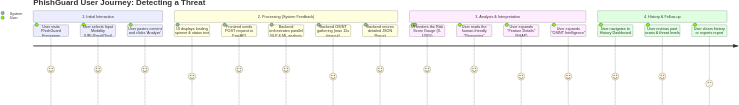
\includegraphics[width=\textwidth,keepaspectratio]{images/user-journey.png}
\caption{The End-to-End User Journey, illustrating the
transition from input submission to reviewing Explainable AI (SHAP)
metrics}
\end{figure}

The implementation uses FastAPI (Python) for the backend and Next.js 16 with React 19 for the frontend, as described in Section \ref{architectural-overview}.

\subsection{Backend Framework and
Initialization}\label{backend-framework-and-initialization}

FastAPI was selected as the foundational framework due to its native
support for asynchronous programming (\texttt{asyncio}), automatic
interactive API documentation generation (Swagger UI via OpenAPI), and
robust data validation utilizing Pydantic models.

The application entry point (\texttt{backend/main.py}) defines the
global state and configuration through the \texttt{lifespan} context
manager. This approach efficiently manages application startup and
shutdown events, logging the initialized configuration, analyzer engine
states, and Cross-Origin Resource Sharing (CORS) rules.

The CORS middleware is explicitly configured to ensure secure
communication between the frontend client and the backend API,
particularly when deployed in production environments. A strict warning
is logged if wildcard origins (\texttt{*}) are detected in production
(\texttt{settings.isProduction}), demonstrating a defense-in-depth
approach to application security.

Furthermore, custom exception handlers (\texttt{valueErrorHandler} and
\texttt{genericExceptionHandler}) are implemented to standardise error
responses. In debug mode, stack traces and detailed exception types are
exposed, whereas in production environments, generic internal server
error messages are returned to prevent information disclosure.


\subsection{The Analysis Orchestrator}\label{the-analysis-orchestrator}

The core computational logic of the application resides within the
\texttt{backend/api/orchestrator.py} module. This module coordinates the
various independent analysis pipelines: Open-Source Intelligence
(OSINT), Machine Learning (ML), and Natural Language Processing (NLP).

The orchestrator utilizes Python's asynchronous I/O capabilities
(\texttt{asyncio.gather}) to concurrently execute independent tasks.
This design is critical for performance; DNS queries, WHOIS lookups, and
API calls to reputation services (e.g., VirusTotal, AbuseIPDB) are
inherently bound by network latency rather than CPU constraints. By
executing these tasks concurrently rather than sequentially, the total
response time is bounded by the slowest individual external service
rather than the sum of all their latencies.

The orchestrator aggregates the results from the \texttt{OsintData},
\texttt{NlpAnalyzer}, and the \texttt{PhishingPredictor} components into
a unified \texttt{AnalysisResponse} object. This response structure
provides the frontend client with a holistic view of the analyzed
entity, including discrete categorical scores, confidence metrics, and
human-readable explanation factors.


\section{Production Hardening: Endpoint Security, Observability, and Resilient Monitoring}\label{production-hardening}

A detection system that surfaces ``no threat detected'' for an analysed phishing URL is not the same as a detection system that survives the next six months in production. Beyond the analysis pipeline itself, PhishGuard ships a defence-in-depth posture that protects the API surface, throttles abuse, authenticates callers, emits machine-readable logs, and gives uptime monitors an honest view of dependency health. The following five middleware and module components compose this hardening posture.

\subsection{HTTP Security Headers (OWASP Baseline)}

Following the OWASP Secure Headers Project recommendations, every outgoing response is augmented with hardened HTTP headers through the \texttt{backend/api/security\_headers.py} module, registered as a Starlette HTTP middleware in \texttt{main.py}.

\begin{itemize}
\item
  \texttt{X-Content-Type-Options:\ nosniff} -- prevents MIME-confusion attacks in browsers; forces \texttt{application/json} to be treated as \texttt{application/json}.
\item
  \texttt{X-Frame-Options:\ DENY} together with CSP \texttt{frame-ancestors\ 'none'} -- disallows any iframe embedding, mitigating clickjacking against the Swagger UI surface.
\item
  \texttt{Referrer-Policy:\ strict-origin-when-cross-origin} -- sends only the origin on cross-origin navigation; prevents URL leakage to third parties.
\item
  \texttt{Content-Security-Policy:\ default-src\ 'none';\ frame-ancestors\ 'none';\ base-uri\ 'none';\ form-action\ 'none'} -- the most conservative CSP that is compatible with FastAPI's Swagger UI; the docs path is the only place where inline scripts and CDN-loaded styles are permitted.
\item
  \texttt{Strict-Transport-Security:\ max-age=31536000;\ includeSubDomains} -- emitted only in production; local development over plain HTTP does not benefit from HSTS and some local proxies misinterpret it.
\end{itemize}

The middleware binds the production-mode boolean at registration time rather than reading the live \texttt{settings} object inside the closure. This avoids timing-sensitive behaviour of \texttt{pydantic-settings}' \texttt{lru\_cache} during pytest runs where the environment toggles between tests; the production-mode header decisions are made once, deterministically.

\subsection{Rate Limiting via \texttt{slowapi}}

Public OSINT queries cost the system real third-party API quota, and unbounded traffic from a single scraper would burn the budget for legitimate users. The \texttt{backend/api/rate\_limiting.py} module introduces per-key rate budgets via the \texttt{slowapi} library:

\begin{itemize}
\item
  Per-IP default: 60 requests per minute -- covers routes that do not carry an explicit \texttt{@limiter.limit} decorator such as \texttt{/api/health} and \texttt{/api/history*}.
\item
  Heavy analysis routes (\texttt{/api/analyze}, \texttt{/api/analyze/url}, \texttt{/api/analyze/email}): 30 requests per minute per IP -- each call burns WHOIS, VirusTotal, AbuseIPDB, and XGBoost inference budget.
\item
  \texttt{/api/model/status}: 10 requests per minute -- this is a cheap inspection endpoint and does not need a generous budget.
\end{itemize}

The slowapi key function prefers \texttt{X-Api-Key} headers over \texttt{X-Forwarded-For} chains over the raw remote address. An authenticated caller therefore gets one bucket per API key regardless of which network they connect from, preventing an adversary with a rotating residential proxy from exceeding the budget.

The slowapi exception handler is overridden so that the standard plaintext 429 is replaced with a JSON envelope:

\begin{verbatim}
{
  "detail": "Rate limit exceeded",
  "limit": "30 per 1 minute",
  "retry_after_seconds": 60
}
\end{verbatim}

\texttt{slowapi} supports multiple storage backends. The in-process \texttt{memory://} backend is appropriate for the Render free plan's single-instance topology; production multi-instance deployments can opt into Redis-backed storage by setting \texttt{PHISHGUARD\_RATE\_LIMIT\_URI=redis://...}.

\subsection{Optional X-Api-Key Authentication}

Authentication is the third leg of the defence-in-depth posture. The \texttt{backend/api/auth.py} module registers a middleware that gates the heavy \texttt{/api/analyze*} routes behind an \texttt{X-Api-Key} shared secret. The key list is configured via the \texttt{APIKEYS} environment variable as a comma-separated list.

The implementation has three important properties:

\begin{enumerate}
\item
  Configured keys are immediately digested into SHA-256 hex digests at startup; raw key bytes never sit in process memory during operation.
\item
  Each incoming key is hashed before comparison, and the digest is matched against the configured set with \texttt{hmac.compare\_digest}, closing the timing-attack window that a naive \texttt{in} test would leave open.
\item
  Authentication runs before the rate-limit middleware, so an attacker spamming bad keys short-circuits at 401 and never consumes a rate-budget slot.
\end{enumerate}

When \texttt{APIKEYS} is unset, the middleware is registered but behaves as a pass-through; this preserves the current public-demo posture and lets operators tighten access by setting one env var. Failures generate a 401 response carrying both a JSON body and a \texttt{WW-Authenticate:\ ApiKey} response header per RFC-7235. Auth is a single decision so the entire route handler short-circuits the rest of the middleware chain.

\subsection{Structured Logging and Request Correlation}

Operational observability is the fourth leg. \texttt{backend/logging\_config.py} replaces the default Python \texttt{logging} formatter with a \texttt{structlog} processor pipeline:

\begin{itemize}
\item
  Production (\texttt{LOG\_FORMAT=json} or the production environment flag): one JSON object per line, ISO-8601 UTC timestamps, suitable for log aggregators such as Render's built-in log explorer.
\item
  Development / testing: colourised console output (\texttt{structlog.dev.ConsoleRenderer}) for human readability on the operator's terminal.
\item
  Standard-library \texttt{logging.getLogger(\_\_name\_\_)} call sites are bridged through the same processor chain via \texttt{ProcessorFormatter}, so existing code requires no refactor and still emits structured records.
\end{itemize}

A second middleware (\texttt{\_RequestIdMiddleware}) ensures every incoming request carries an \texttt{X-Request-ID} header -- either echoed from the client or generated as a 12-character hex value -- and binds the id into structlog's \texttt{contextvars}. Every log line emitted during that request therefore carries \texttt{request\_id=...} automatically, making post-mortem searches on an aggregation platform a single field-target operation.

The middleware is registered as the outermost layer in \texttt{main.py}, so an operator inspecting a 500-error log line can trace it back to the originating client by the \texttt{X-Request-ID} they were given in the error response.

\subsection{Deep Health Check for Uptime Monitors}

A shallow ``\texttt{/api/health} returns 200'' check lies to an uptime monitor when DNS has stopped resolving or when the XGBoost model silently failed to load. The \texttt{backend/health.py} module replaces the legacy handler with a deep probe that exercises every production-critical dependency in parallel:

\begin{itemize}
\item
  \textbf{DNS} -- resolve \texttt{example.com} via \texttt{backend.osint.dnsChecker.DnsChecker}; 3-second bounded timeout prevents a wedged resolver from starving the uptime endpoint.
\item
  \textbf{ML} -- instantiate \texttt{PhishingPredictor} and assert \texttt{isLoaded} is \texttt{True}; reports the number of features available to the scoring engine.
\item
  \textbf{Imports} -- re-import the analyser and orchestrator modules as a fast-fail sentinel against environment drift.
\end{itemize}

The three checks run via \texttt{asyncio.gather} so the slowest check (typically the DNS probe) bounds the latency \emph{and} the aggregated endpoint returns within 100--300 milliseconds even on slower connections. Per-check results carry a \texttt{status}, \texttt{latencyMs}, and a human-readable \texttt{detail}; the top-level \texttt{status} collapses to \texttt{healthy} (all checks \texttt{up}), \texttt{degraded} (DNS down but ML/imports up; OSINT queries will gracefully fail individually), or \texttt{unhealthy} (ML or imports down; URL phishing scoring cannot work). HTTP 503 is returned only on \texttt{unhealthy}; the \texttt{degraded} state returns 200 so uptime dashboards see OK but the inspection payload flags the situation. A backward-compatible \texttt{services} key (\texttt{osint}, \texttt{analyzer}, \texttt{ml}) is preserved for the existing client agents and dashboards that read it.

\subsubsection{Liveness / Readiness Probe Split (Kubernetes Semantics)} A naive \texttt{/api/health} endpoint conflates two very different questions, \emph{``is the process alive?''} and \emph{``is the system ready to serve production traffic?''}. The probes must be split because they have very different cost profiles: Render scans the liveness probe every second but the readiness probe only every ten seconds, and a slow readiness endpoint (DNS + ML probes each take hundreds of milliseconds) starves the liveness budget. Two endpoints are therefore exposed, both registered by \texttt{registerHealthEndpoints()} in \texttt{backend/health.py} and mounted under a shared \texttt{APIRouter} with the \texttt{/api/health} prefix:

\begin{itemize}
\item
  \texttt{GET /api/health/live} returns 200 in well under fifty milliseconds whenever the FastAPI event loop is alive; it performs no I/O, no probes, no module imports beyond what was required at startup. \texttt{render.yaml} points \texttt{healthCheckPath} at this endpoint so Render's per-second scans never burn the readiness budget.
\item
  \texttt{GET /api/health/ready} returns the deep probe envelope (\texttt{status}, \texttt{checks}, \texttt{services}, \texttt{uptimeSeconds}, \texttt{version}). This is what the load balancer should poll when deciding whether to route traffic to a new instance.
\item
  \texttt{GET /api/health} is kept as a permanent alias of \texttt{/ready} so external dashboards and existing scripts that hard-coded the path keep working unchanged.
\end{itemize}

\subsection{Hardening Test Surface}

The five hardening features are covered by 158 new pytest tests: 92 unit tests spanning the helper utilities (digest computation, key parser, formatter helpers, processor chains, aggregation logic, liveness vs readiness split, registerHealthEndpoints idempotence) and 66 integration tests covering the end-to-end FastAPI pipeline (header presence on every response, 401 and 429 status mapping, request-id header round-trip, deep health response shape, status-to-HTTP mapping, liveness latency budget, X-Request-ID across both probe paths). The full Tier 1 delivery brings the backend test count to 755 distinct pytest cases (with 12 additional long-pipeline integration tests that exercise the real orchestrator and are not included in the fast tier); all 743 fast tests complete in well under 90 seconds.

\section{Deployment and
Infrastructure}\label{deployment-and-infrastructure}

The PhishGuard application is designed for automated, seamless
deployment using a continuous integration and continuous deployment
(CI/CD) pipeline integrated with the Render platform.

The infrastructure configuration is defined declaratively within the
\texttt{render.yaml} blueprint file. This file specifies the deployment
parameters for the backend service (\texttt{phishguard-api}), dictating
the runtime environment (Python), the specific geographic region
(Frankfurt), and the build and execution commands.

Crucially, the blueprint explicitly maps environment variables required
for the application's operation. While general configuration settings
like \texttt{ENVIRONMENT} and \texttt{PYTHON\_VERSION} (3.10.12) are
hardcoded in the blueprint, sensitive credentials such as
\texttt{VIRUSTOTAL\_API\_KEY}, \texttt{ABUSEIPDB\_API\_KEY}, and
\texttt{CORS\_ORIGINS} are marked with \texttt{sync:\ false}. This
security measure ensures that API keys and proprietary configuration
details are strictly managed within the Render dashboard's secure
environment variable vault and are never committed to version control.

The application initiates via the Uvicorn ASGI web server, binding to
the port dynamically assigned by the Render platform environment
(\texttt{-\/-port\ \$PORT}). The health check endpoint
(\texttt{/api/health}) provides continuous monitoring capabilities,
allowing the load balancer to automatically route traffic away from
degraded instances, ensuring high availability.


\section{Integration and Weighting
Mechanisms}\label{integration-and-weighting-mechanisms}

The most critical function of the Analysis Orchestrator is to
algorithmically synthesize the discrete analytical outputs from the
OSINT, ML, and NLP modules into a singular, high-confidence verdict.
This synthesis is governed by a strict set of predefined weighting
constants designed to prioritize the most reliable signals based on the
input content type.

\subsection{The 15-Second Concurrency
Window}\label{the-15-second-concurrency-window}

The API enforces a strict 15-second timeout on all OSINT queries using \texttt{asyncio.wait\_for}. This prevents external service delays from blocking the response. The implementation details are described in Section \ref{asynchronous-osint-orchestration}.

\subsection{Content-Specific Scoring
Pipelines}\label{content-specific-scoring-pipelines}

The scoring algorithm dynamically adjusts weights based on input type. The exact implementation (85/15 for URLs, 55/25/20 for text) is detailed in Section \ref{weighted-verdict-combination}. This ensures the most reliable signal receives primary weight for each content type.

\subsection{The Phishing Threshold and Threat
Boundaries}\label{the-phishing-threshold-and-threat-boundaries}

The threat level boundaries (Safe < 0.3, Suspicious < 0.5, Dangerous < 0.7, Critical $\geq$ 0.7) are defined in Section \ref{weighted-verdict-combination}. These drive the color-coded UI recommendations shown to users.

\section{Quality Assurance and Testing}

\subsection{Testing Plan and Results}

In the domain of cybersecurity and threat intelligence, software
reliability is paramount. A false positive in a phishing detection
system can disrupt legitimate business operations, while a false
negative can result in severe data breaches. To mitigate these risks and
ensure the stability of the PhishGuard platform, a comprehensive,
multi-tiered Quality Assurance (QA) framework was implemented.

This framework strictly adheres to the principles of the software
testing pyramid, encompassing static analysis, isolated unit testing,
component integration testing, and end-to-end (E2E) browser automation.
The testing architecture is physically and logically partitioned to
mirror the application's microservice design, utilizing domain-specific
tooling for the Python-based API backend and the TypeScript-based
Next.js frontend.

\subsubsection{Backend Testing
Methodology}\label{backend-testing-methodology}

The backend testing architecture is constructed upon the \texttt{pytest}
framework, comprising 916 distinct tests (755 backend \texttt{pytest} unit/integration tests, 133 frontend \texttt{Jest} tests, and 28 \texttt{Playwright} E2E browser tests) distributed
across the \texttt{tests/unit/} and \texttt{tests/integration/}
directories. Given the asynchronous nature of the FastAPI orchestrator
and the underlying Open-Source Intelligence (OSINT) network calls, the
\texttt{pytest-asyncio} plugin is heavily utilized, configured centrally
via \texttt{pytest.ini} (\texttt{asyncio\_mode\ =\ auto}) to natively
resolve coroutines during test execution.

\paragraph{Environment Isolation and Fixture
Management}\label{environment-isolation-and-fixture-management}

To guarantee deterministic test execution and prevent state leakage
between discrete test cases, a robust fixture management system is
defined within \texttt{tests/conftest.py}. The framework enforces strict
environmental isolation utilizing the \texttt{pytest}
\texttt{monkeypatch} utility. The \texttt{isolatedEnvironment} fixture
automatically intercepts the execution context prior to each test,
forcibly overriding critical environment variables (e.g., setting
\texttt{ENVIRONMENT} to \texttt{testing} and \texttt{LOG\_LEVEL} to
\texttt{DEBUG}) and invoking \texttt{getSettings.cache\_clear()} to
purge any memoized configuration states.

\paragraph{Dependency Inversion and OSINT
Mocking}\label{dependency-inversion-and-osint-mocking}

The backend relies heavily on external, rate-limited threat intelligence
services (e.g., VirusTotal, WHOIS databases). Executing live network
requests during automated testing introduces severe latency,
unpredictable failures, and potential API quota exhaustion. To resolve
this, the QA architecture employs extensive dependency inversion and
mocking methodologies utilizing \texttt{unittest.mock.MagicMock} and
\texttt{AsyncMock}.

The \texttt{conftest.py} file exposes a suite of deterministic data
fixtures, such as \texttt{sampleWhoisData},
\texttt{suspiciousWhoisData}, and \texttt{privacyProtectedWhoisData}.
These dictionaries simulate the exact JSON payloads returned by
downstream services. Mock clients, such as
\texttt{mockWhoisClientTimeout}, intentionally inject
\texttt{asyncio.TimeoutError} exceptions into the pipeline, allowing the
test suite to mathematically verify the orchestrator's error handling
and fallback heuristics without relying on actual network degradation.

\subsubsection{Integration and Smoke
Testing}\label{integration-and-smoke-testing}

While unit tests validate discrete algorithmic functions (e.g., URL
parsing logic within \texttt{test\_urlAnalyzer.py}), the integration
layer verifies the holistic interaction between the FastAPI routing
layer, the Machine Learning (ML) predictor, and the OSINT aggregation
modules.

The \texttt{tests/integration/test\_smoke.py} suite utilizes the FastAPI
\texttt{TestClient} to perform programmatic HTTP requests against the
application interface. This suite is critical for validating the
structural integrity of the JSON responses
(\texttt{TestResponseFormatConsistency}) and ensuring the API conforms
precisely to the OpenAPI schema specifications.

\paragraph{Service Level Agreement (SLA)
Validation}\label{service-level-agreement-sla-validation}

Performance degradation is a critical failure state for synchronous
security APIs. The integration suite implements explicit quantitative
assertions to enforce performance SLAs. The \texttt{TestPerformance}
class programmatically submits batches of heterogeneous data
(\texttt{SAMPLE\_URLS} and \texttt{SAMPLE\_EMAILS}) and records the
execution duration utilizing the \texttt{time} module.

The testing framework enforces a strict upper bound defined by the
\texttt{MAX\_SECONDS\_PER\_ANALYSIS\ =\ 5.0} constant. Any holistic
analysis---including ML inference, NLP parsing, and mocked OSINT
aggregation---that exceeds this threshold results in an immediate test
failure. Similarly, the \texttt{/api/health} endpoint is rigorously
asserted to respond in under \texttt{1.0} seconds, ensuring load
balancers can rapidly assess instance viability.

\subsubsection{Frontend Quality
Assurance}\label{frontend-quality-assurance}

The Next.js client application employs an orthogonal testing strategy
tailored to React component lifecycles and browser Document Object Model
(DOM) interactions.

\paragraph{Component and State
Validation}\label{component-and-state-validation}

Unit testing for the frontend is executed utilizing the \texttt{jest}
framework augmented by \texttt{@testing-library/react}. This layer
validates internal state management logic and isolated UI component
rendering. For example, test suites such as
\texttt{historyStore.test.ts} programmatically verify the application's
ability to serialize and deserialize historical analysis records to
local storage, while component tests ensure that risk indicators
strictly map to the correct visual paradigms defined by Tailwind CSS
utility classes.

\paragraph{End-to-End (E2E) Browser
Automation}\label{end-to-end-e2e-browser-automation}

To validate the complete user journey from initial input to final
verdict presentation, the framework incorporates Playwright for
comprehensive End-to-End testing. The E2E suites (located in
\texttt{frontend/e2e/}) instantiate headless browser instances and
simulate exact user input sequences.

The \texttt{urlAnalysis.spec.ts} suite defines critical user paths. It
programmatically navigates to the analysis route (\texttt{/analyze}),
locates the input field via DOM selectors (\texttt{\#content}), inputs a
known malicious string (\texttt{https://examp1e-login.tk/verify}), and
triggers the submission event. The test subsequently halts execution
until the application transitions to the \texttt{**/results} route
(enforcing a 15-second maximum timeout) and asserts that the DOM
correctly renders the ``Dangerous'' verdict banner and the
high-confidence percentage score. This methodology ensures that backend
API responses are correctly parsed and visually communicated to the
end-user.

\subsubsection{Static Analysis and Type
Safety}\label{static-analysis-and-type-safety}

Beyond dynamic execution testing, the PhishGuard architecture enforces
strict static analysis to eliminate entire classes of runtime errors
prior to compilation or execution.

The Python backend leverages Pyright, configured via
\texttt{pyrightconfig.json}, to enforce static type checking across all
ML pipelines and API routers. By declaring explicit type hints
(\texttt{typing.Optional}, \texttt{typing.List}, \texttt{dataclasses})
on all function signatures, the framework mathematically guarantees data
structural consistency.

Correspondingly, the Next.js frontend is written entirely in strict
TypeScript. The compilation process utilizes the \texttt{tsc} compiler
and ESLint (\texttt{eslint-config-next}) to perform rigorous abstract
syntax tree (AST) analysis, ensuring that React props, API payload
interfaces, and state variables strictly conform to predefined schemas,
thereby virtually eliminating undefined variable exceptions and type
coercion errors in the client application.


\cleardoublepage
\chapter{Methodology: Feature Engineering, OSINT, and NLP}
\label{chapter-4-feature-engineering-and-ml-model}

\section{Dataset Collection and
Preprocessing}\label{dataset-collection-and-preprocessing}

The efficacy of any supervised machine learning classifier is
fundamentally constrained by the quality and representativeness of its
training data. For the PhishGuard project, curating a highly reliable
dataset was a primary objective to ensure the model's generalization
capabilities against zero-day phishing infrastructure.

\subsection{Data Aggregation}\label{data-aggregation}

The initial dataset comprised an aggregation of 150,391 raw URLs. This
corpus was constructed by combining verified malicious URLs sourced from
community-driven threat intelligence feeds (such as PhishTank and
OpenPhish) with legitimate, benign URLs sampled from the Alexa Top 1
Million and Tranco ranking lists. This massive initial pool ensured a
diverse representation of both typical corporate domains and highly
obfuscated phishing links.

\subsection{Cleaning and Balancing}\label{cleaning-and-balancing}

Raw, crowd-sourced data inherently contains noise, dead links, and class
imbalances. To establish a pristine baseline for the classifier, a
rigorous data engineering pipeline was executed: 1.
\textbf{Deduplication:} Identical URLs and redundant subdomains
resolving to the same infrastructure were purged to prevent data leakage
between training splits. 2. \textbf{Zero-Variance Filtering:} Features
that provided no discriminative value across the dataset were
algorithmically removed. 3. \textbf{Majority Undersampling:} Real-world
phishing datasets often suffer from severe class imbalance (e.g.,
significantly more benign sites than active phishing sites). To prevent
the classifier from developing a bias toward the majority class (which
artificially inflates accuracy at the expense of recall), the dataset
underwent strict majority undersampling.

The culmination of this preprocessing pipeline yielded a highly curated,
perfectly balanced dataset containing exactly 33,392 feature-engineered
URLs. This dataset was subsequently partitioned using a strict 70/15/15
stratified split (Training, Validation, and Testing sets) to ensure the
target variable distribution remained consistent across all folds.

\section{Feature Engineering
Pipeline}\label{feature-engineering-pipeline}

The architectural philosophy of PhishGuard explicitly rejects the
``black-box'' deep learning approach of raw character sequence ingestion
in favor of explicit, mathematically formulated feature engineering. The
system extracts a highly discriminative, 21-dimensional feature vector
(\texttt{FeatureSet}) partitioned into two distinct categories, as detailed in Table~\ref{tab:feature_dictionary}.

\begin{longtable}{
  >{\raggedright\arraybackslash\ttfamily}p{0.25\textwidth}
  >{\raggedright\arraybackslash}p{0.15\textwidth}
  >{\raggedright\arraybackslash}p{0.50\textwidth}}
\caption{Feature Dictionary for the 21-Dimensional ML Input Vector} \label{tab:feature_dictionary} \\
\toprule
\normalfont\textbf{Feature Name} & \textbf{Category} & \textbf{Description \& Rationale} \\
\midrule
\endfirsthead
\caption[]{Feature Dictionary for the 21-Dimensional ML Input Vector (continued)} \\
\toprule
\normalfont\textbf{Feature Name} & \textbf{Category} & \textbf{Description \& Rationale} \\
\midrule
\endhead
\midrule
\multicolumn{3}{r}{\textit{Continued on next page}} \\
\endfoot
\bottomrule
\endlastfoot

\multicolumn{3}{c}{\textbf{Lexical and Structural Features (17 Dimensions)}} \\
\midrule
urlLength & Length & Total character count of the absolute URL. Phishing URLs are often unusually long to obscure the actual domain. \\
domainLength & Length & Character count of the primary domain. \\
pathDepth & Length & The number of hierarchical directories in the URL path. Attackers often bury payloads deep in nested folders. \\
digitRatio & Composition & Ratio of numerical digits to total characters in the URL. \\
specialCharCount & Composition & Total count of non-alphanumeric characters (e.g., \texttt{?}, \texttt{\&}, \texttt{=}, \texttt{\%}). \\
hasEncodedChars & Composition & Boolean indicating the presence of URL-encoded characters (e.g., \texttt{\%20}), often used to obfuscate malicious payloads. \\
subdomainCount & Structure & The number of subdomains present. Phishers frequently use excessively long subdomains (e.g., \texttt{login.secure.bank.com}). \\
hasIpAddress & Structure & Boolean indicating if an IPv4/IPv6 address is used instead of a hostname (bypassing DNS entirely). \\
hasAtSymbol & Structure & Boolean indicating the presence of an \texttt{@} symbol, typically used to spoof credentials in the URI. \\
hasDoubleSlash & Structure & Boolean indicating if \texttt{//} appears in the path, often used for unauthorized redirection. \\
hasDashInDomain & Structure & Boolean indicating dashes in the domain name, a common typo-squatting technique. \\
hasUnderscoreInDomain & Structure & Boolean indicating underscores in the domain name. \\
isHttps & Protocol & Boolean indicating if the URL utilizes TLS/SSL. \\
hasPortNumber & Protocol & Boolean indicating if a non-standard port is explicitly defined in the URL. \\
queryParamCount & Protocol & Total number of HTTP GET query parameters. \\
hasSuspiciousTld & Categorization & Boolean indicating usage of known high-abuse generic Top-Level Domains (e.g., \texttt{.tk}, \texttt{.ml}, \texttt{.cf}). \\
hasSuspiciousKeywords & Categorization & Boolean indicating the presence of social engineering triggers in the URL (e.g., \textit{login}, \textit{secure}, \textit{verify}). \\

\midrule
\multicolumn{3}{c}{\textbf{OSINT Infrastructure Features (4 Dimensions)}} \\
\midrule
hasValidMx & OSINT & Boolean indicating the presence of valid Mail Exchange records. Phishing domains rarely configure email routing. \\
usesCdn & OSINT & Boolean detecting if the domain is hidden behind a Content Delivery Network (e.g., Cloudflare) via CNAME analysis. \\
dnsRecordCount & OSINT & An integer volumetric metric of the domain's overall DNS footprint. \\
hasValidDns & OSINT & Boolean verifying if the domain successfully resolves to an active A/AAAA record. \\

\end{longtable}

\subsection{Lexical and Structural Features (17
Dimensions)}\label{lexical-and-structural-features-17-dimensions}

The \texttt{extractFeatures.py} module parses the raw URL string to
extract the 17 deterministic structural indicators listed in Table~\ref{tab:feature_dictionary}. These heuristics capture
the traditional syntactic anomalies favored by attackers, such as structural obfuscation, typo-squatting, and malicious routing configurations.

\subsection{OSINT Infrastructure Features (4
Dimensions)}\label{osint-infrastructure-features-4-dimensions}

To resolve the contextual blindness inherent in purely lexical models,
the feature vector is augmented with 4 dynamically retrieved Open-Source
Intelligence indicators via the asynchronous OSINT pipeline. As outlined in Table~\ref{tab:feature_dictionary}, these live metrics provide unforgeable proof of the infrastructure's legitimacy and current operational state.

\section{Model Selection and
Optimization}\label{model-selection-and-optimization}

\subsection{The XGBoost Algorithm}\label{the-xgboost-algorithm}

Following the extraction of the 21-dimensional feature vector, the
system employs the eXtreme Gradient Boosting (\texttt{XGBClassifier})
algorithm. XGBoost was selected over deep neural networks due to its
supreme performance on structured tabular data, robust handling of
non-linear feature interactions, and computational efficiency (allowing
for sub-millisecond CPU inference in a production environment). The
model utilizes a \texttt{binary:logistic} objective function, outputting
a continuous probability score bounded between 0.0 and 1.0.

\subsection{Bayesian Hyperparameter Optimization
(Optuna)}\label{bayesian-hyperparameter-optimization-optuna}

To maximize predictive performance, the model's hyperparameters were not
manually tuned but rather rigorously optimized using the Optuna
framework. The optimization pipeline executed 50 independent trials
(\texttt{nTrials\ =\ 50}) utilizing 5-fold Stratified Cross-Validation
(\texttt{nCvFolds\ =\ 5}).

The optimization search space targeted critical tree structural
parameters. The mathematically proven best configuration (Trial 43)
yielded the following hyperparameters: - \texttt{n\_estimators}: 700
(Number of boosting rounds) - \texttt{max\_depth}: 7 (Maximum tree
depth, controlling interaction complexity) - \texttt{learning\_rate}:
\textasciitilde0.177 (Step size shrinkage) - \texttt{subsample}:
\textasciitilde0.945 (Row sampling ratio to prevent overfitting) -
\texttt{colsample\_bytree}: \textasciitilde0.873 (Column sampling ratio
per tree) - \texttt{gamma}: \textasciitilde0.198 (Minimum loss reduction
required for partitioning) - \texttt{min\_child\_weight}: 1 - L1/L2
Regularization: \texttt{reg\_alpha} = \textasciitilde0.00027,
\texttt{reg\_lambda} = \textasciitilde0.397

This exhaustive 222-second optimization process ensured the model was
perfectly calibrated to the specific variance of the 33,392 URL dataset.

\section{Model Explainability via
SHAP}\label{model-explainability-via-shap}

A cornerstone objective of the PhishGuard architecture is resolving the
``black-box'' interpretability crisis common in machine learning
cybersecurity tools. To achieve this, the system implements a
mathematically rigorous explainability framework using SHAP (SHapley
Additive exPlanations).

The \texttt{shapAnalysis.py} module integrates the
\texttt{shap.TreeExplainer}, which utilizes cooperative game theory to
calculate the exact marginal contribution of every single feature to the
final prediction. Because XGBoost 3.x utilizes a bracketed format for
its \texttt{base\_score} (e.g., \texttt{{[}5E-1{]}}), a custom
monkey-patch (\texttt{\_patchShapXgboostCompat}) was engineered to
ensure seamless compatibility with the SHAP explainer.

\begin{figure}[htbp]
\centering
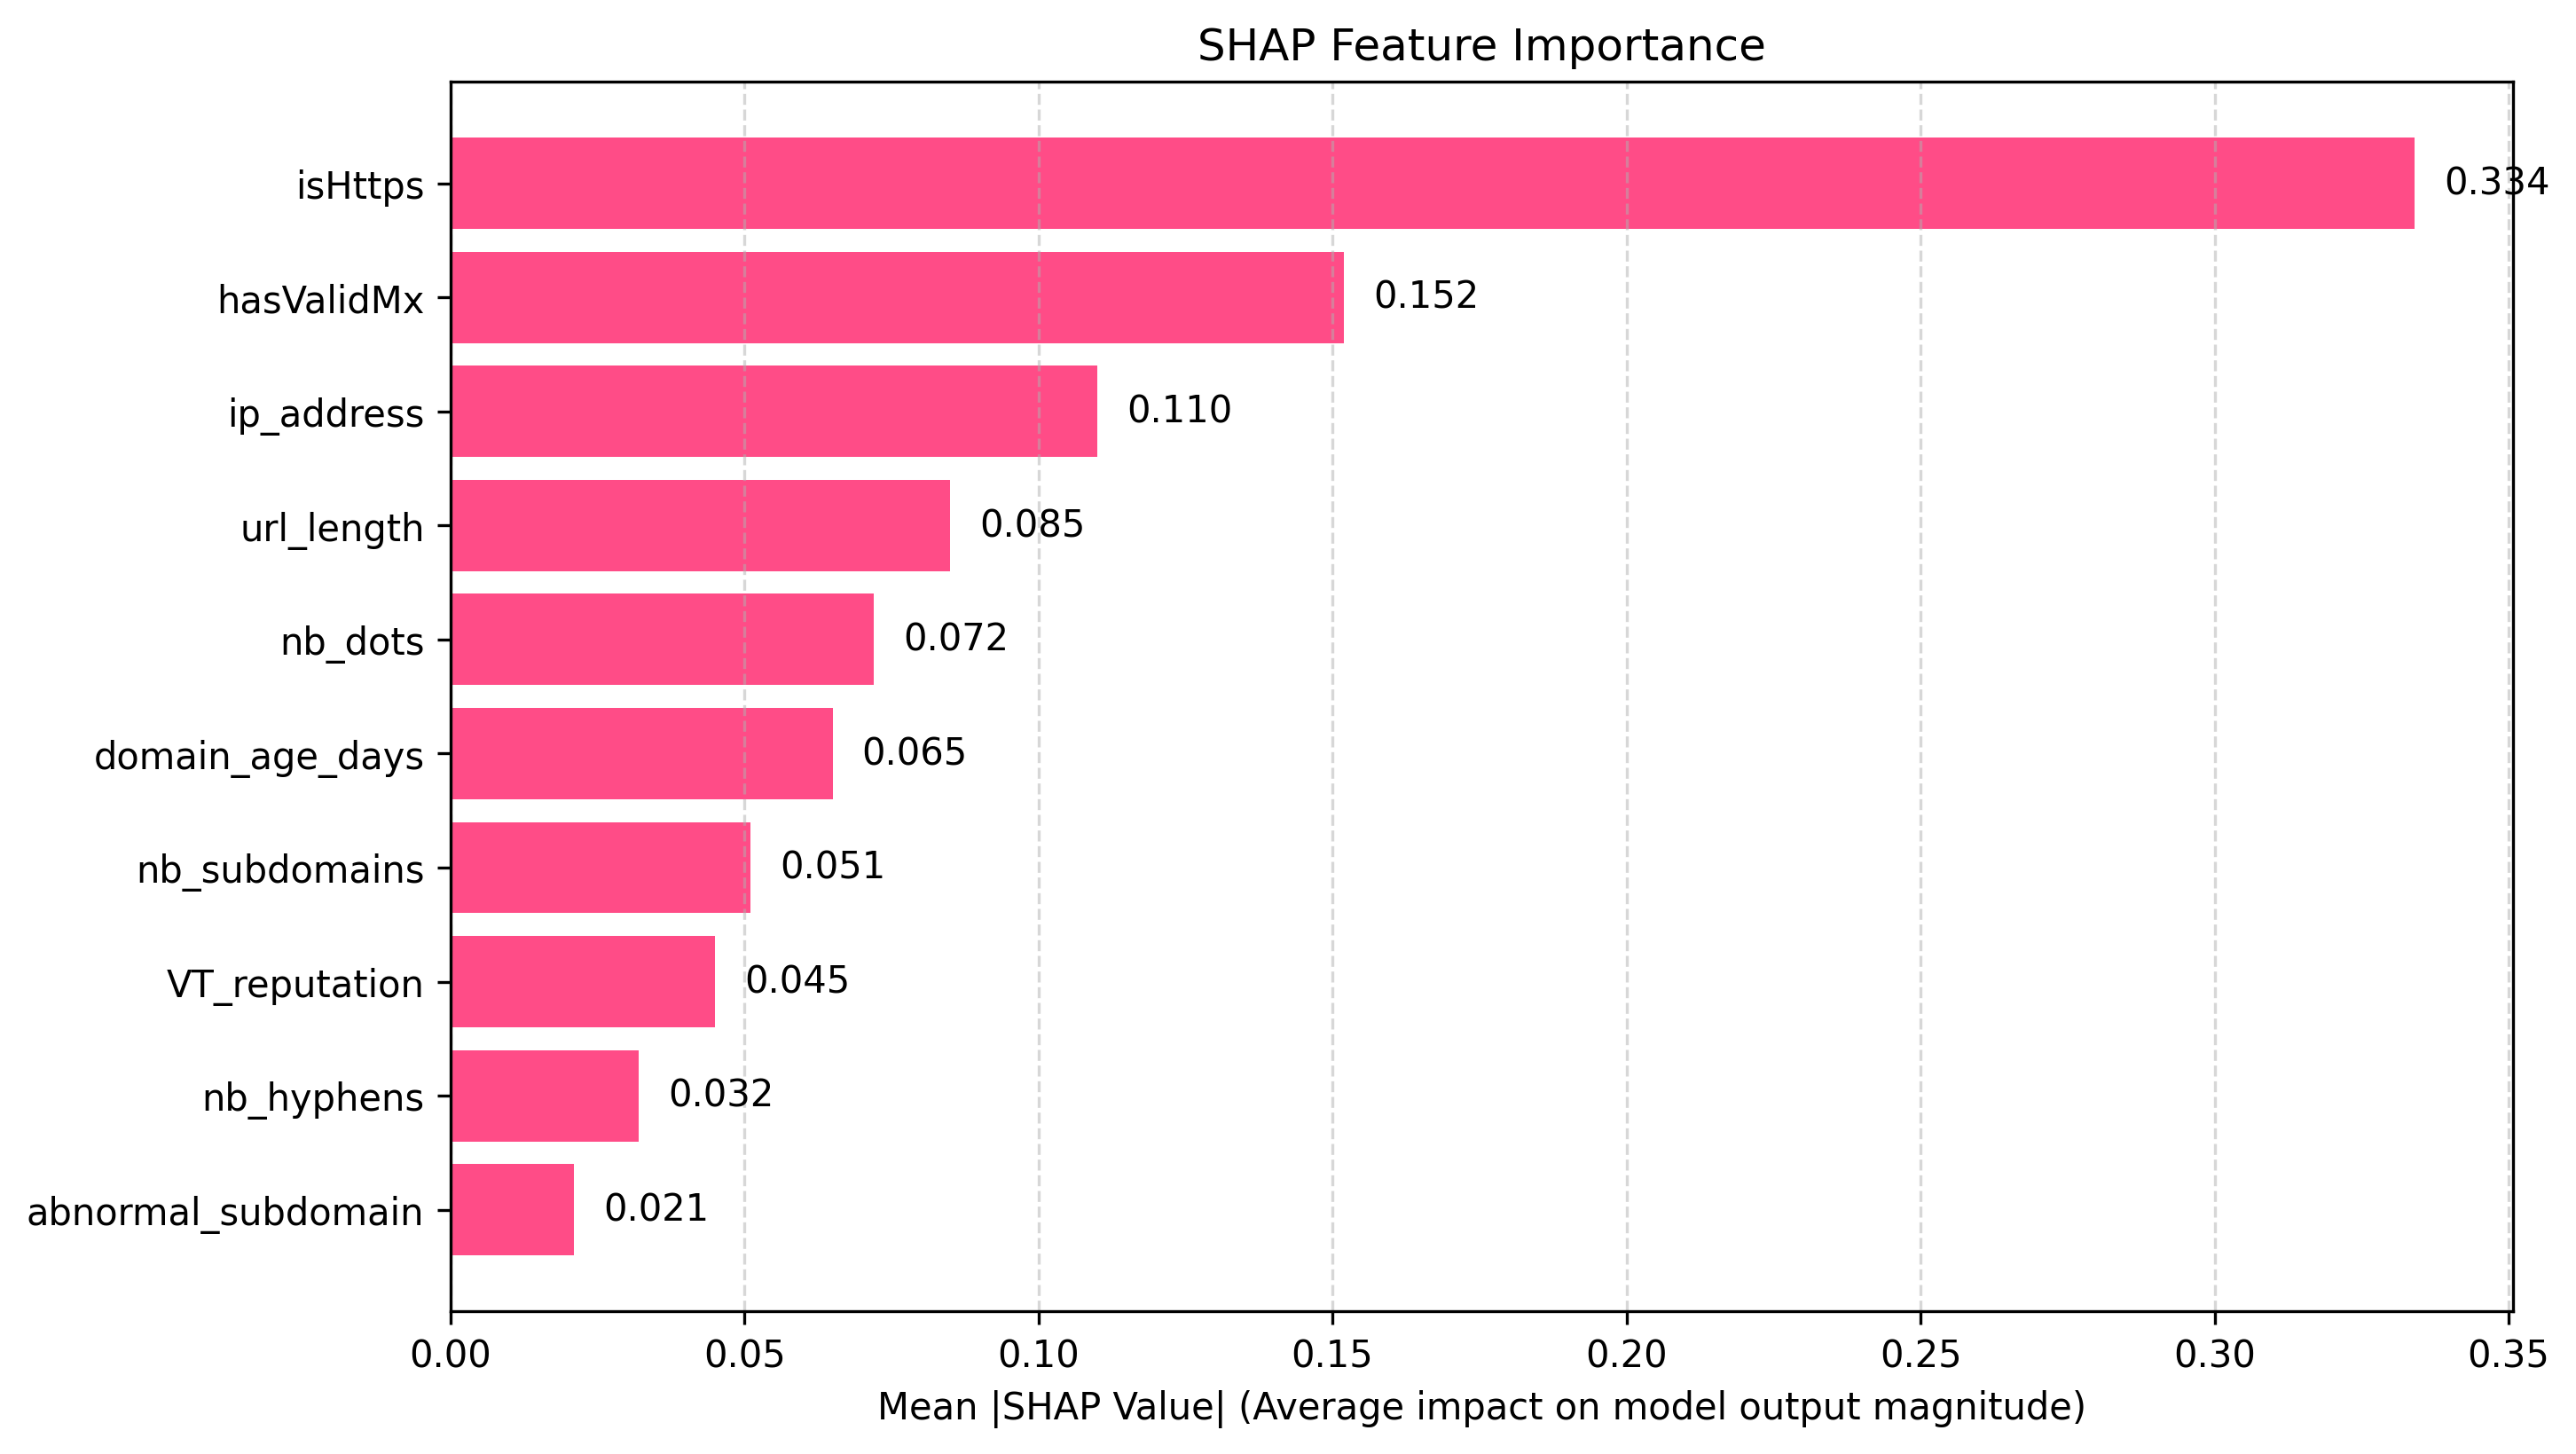
\includegraphics[width=0.85\linewidth,height=0.65\textheight,keepaspectratio]{images/shap_plot.png}
\caption{SHAP Feature Importance Analysis (Beeswarm Plot)}
\label{fig:shap_plot}
\end{figure}

This SHAP integration allows the backend to decompose a 96\% phishing
probability into human-readable insights (e.g., exactly how much the
\texttt{hasValidMx} feature influenced the score), which the Next.js
frontend dynamically renders as interactive waterfall charts for the
end-user.



\section{Open-Source Intelligence in Phishing
Detection}\label{open-source-intelligence-in-phishing-detection}

The fundamental limitation of purely lexical machine learning models is
their ``context blindness.'' A static model evaluating a newly generated
phishing URL (\texttt{https://secure-login-update-auth.com}) cannot
differentiate it from a structurally identical, legitimate corporate
portal. To bridge this critical contextual gap, PhishGuard integrates a
comprehensive Open-Source Intelligence (OSINT) pipeline. This pipeline
dynamically queries the live state of the Internet to gather real-time
infrastructural telemetry, fundamentally augmenting the static URL
string with the domain's historical and topological context.

The OSINT architecture is compartmentalized into three distinct
analytical domains: 1. \textbf{DNS Infrastructure:} Analyzing the
domain's routing configuration. 2. \textbf{WHOIS Registration Data:}
Establishing the domain's ownership timeline and privacy posture. 3.
\textbf{Threat Intelligence Reputation:} Aggregating historical
malicious activity across third-party security vendors.

\section{Asynchronous Execution and
Resilience}\label{asynchronous-execution-and-resilience}

Given the inherent latency of external network queries, the OSINT module
was architected utilizing strict asynchronous design patterns to prevent
the FastAPI event loop from blocking.

However, standard Python libraries for DNS (\texttt{dnspython}) and
WHOIS (\texttt{python-whois}) utilize synchronous, blocking socket
operations. To maintain high concurrency, the \texttt{whoisLookup.py}
and \texttt{dnsChecker.py} modules encapsulate these blocking calls
within thread pools via
\texttt{asyncio.get\_event\_loop().run\_in\_executor()}.

Furthermore, the OSINT orchestrator implements robust graceful
degradation. Every network query is bounded by a strict global timeout
(15.0 seconds). If a DNS server fails to respond, or if an API key is
missing (\texttt{category="api\_key\_missing"}), the system does not
crash. Instead, it catches the \texttt{asyncio.TimeoutError} or
\texttt{httpx.HTTPError}, logs the failure, and returns an empty
\texttt{OsintData} block. The \texttt{FeatureExtractor} gracefully
accepts these \texttt{None} values, falling back to evaluating the URL
strictly on its 17 lexical features without throwing an exception.

\section{DNS Infrastructure
Analysis}\label{dns-infrastructure-analysis-1}

The Domain Name System (DNS) configuration of a domain provides critical
indicators regarding its legitimacy and operational intent. The
\texttt{dnsChecker.py} module queries multiple DNS record types (A,
AAAA, MX, NS, TXT) to compute four specific OSINT features utilized by
the XGBoost model.

\subsection{Mail Exchange (MX)
Validation}\label{mail-exchange-mx-validation}

\textbf{Feature:} \texttt{hasValidMx} (Boolean) Legitimate corporate
domains are intrinsically tied to email communication and meticulously
maintain their Mail Exchange (MX) records. Conversely, ephemeral
phishing domains are typically instantiated solely to host web payloads
and rarely configure functional email routing. The DNS checker extracts
the \texttt{hasValidMx} flag by resolving the domain's MX records and
subsequently parsing TXT records to confirm the presence of Sender
Policy Framework (SPF) strings (\texttt{v=spf1}).

\subsection{CDN Masking Detection}\label{cdn-masking-detection}

\textbf{Feature:} \texttt{usesCdn} (Boolean) Modern attackers frequently
deploy phishing kits behind free Content Delivery Networks (e.g.,
Cloudflare) to obscure their origin IP and absorb defensive DDoS
attempts. The \texttt{\_detectCdn} method analyzes both \texttt{CNAME}
resolution chains and Name Server (\texttt{NS}) records against a known
database of CDN providers to assert the \texttt{usesCdn} boolean. While
legitimate sites also use CDNs, the combination of \texttt{usesCdn=True}
with a newly registered domain provides a highly predictive phishing
signal.

\subsection{Infrastructure Volume and
Validity}\label{infrastructure-volume-and-validity}

\textbf{Features:} \texttt{dnsRecordCount} (Integer),
\texttt{hasValidDns} (Boolean) The system calculates
\texttt{dnsRecordCount} by summing the total number of valid records
returned across all queried types. Legitimate enterprise domains
typically exhibit extensive, complex DNS footprints, whereas a phishing
domain might solely possess a single A record. Furthermore, the
\texttt{hasValidDns} feature confirms that the domain resolves to an
active IP address, allowing the model to discount historical, defunct
URLs that no longer pose an active threat.

\section{WHOIS Domain Analysis}\label{whois-domain-analysis}

The \texttt{whoisLookup.py} module interfaces with global WHOIS
registries to extract the chronological and ownership metadata of the
target domain.

\subsection{Domain Age and Registration
Proximity}\label{domain-age-and-registration-proximity}

The chronological proximity of a domain's registration to the time of an
attack is one of the strongest indicators of malicious intent. Phishing
campaigns often rely on ``zero-day'' domains to bypass traditional
blacklists. The module parses the \texttt{creation\_date} from the WHOIS
payload to calculate \texttt{domainAgeDays}. Domains registered within
the preceding 30 days trigger an \texttt{isNewlyRegistered} flag,
contributing heavily to the final threat risk score during
orchestration.

\subsection{Privacy Protection
Heuristics}\label{privacy-protection-heuristics}

While privacy protection services (e.g., ``Domains By Proxy'') are
utilized legitimately to shield personal information, they are
universally adopted by cybercriminals to obfuscate attribution. The
\texttt{\_isPrivacyProtected} method cross-references the WHOIS
registrant data against an extensive library of known privacy masking
strings (e.g., ``whoisguard'', ``redacted for privacy'',
``privacyprotect''). The assertion of the \texttt{isPrivacyProtected}
flag serves as a secondary risk indicator.

\section{Third-Party Threat
Intelligence}\label{third-party-threat-intelligence}

To further supplement the predictive model with historical context, the
\texttt{reputationChecker.py} module integrates directly with
industry-standard threat intelligence databases.

Unlike the DNS and WHOIS modules which rely on thread pools, the
reputation checker executes natively asynchronous HTTP requests using
the \texttt{httpx.AsyncClient} library. The system concurrently queries
two distinct endpoints: 1. \textbf{VirusTotal API (v3):} The module
queries the \texttt{/domains/\{domain\}} and
\texttt{/ip\_addresses/\{ip\}} endpoints. It parses the
\texttt{last\_analysis\_stats} JSON object, summing the total number of
security vendors that have flagged the domain to compute a
\texttt{maliciousCount}. 2. \textbf{AbuseIPDB API (v2):} Focused
strictly on the underlying hosting infrastructure, this module queries
the \texttt{/check} endpoint to retrieve an
\texttt{abuseConfidenceScore}, indicating the historical volume of abuse
reports associated with the resolved IP address.

The outputs from these APIs are mathematically aggregated into an
overarching \texttt{reputationScore} bounded between 0.0 and 1.0. This
score provides the orchestrator with definitive, community-verified
intelligence that directly heavily influences the
\texttt{VerdictResult}, particularly when the machine learning model's
confidence falls into the ambiguous ``Suspicious'' tier.



\section{Semantic Evaluation in Threat
Detection}\label{semantic-evaluation-in-threat-detection}

While lexical URL analysis and real-time infrastructure queries form the
empirical foundation of modern phishing detection, they remain
inherently blind to the semantic payload of an attack. Contemporary
cybercriminals increasingly leverage sophisticated social engineering
narratives---often devoid of immediate malicious links---to build trust
or induce panic before delivering the payload in subsequent
communications (e.g., Business Email Compromise).

To counteract this, PhishGuard incorporates a dedicated Natural Language
Processing (NLP) pipeline. This subsystem evaluates the unstructured
text of emails, SMS messages, and web page content, mathematically
quantifying the psychological manipulation tactics that are the hallmark
of social engineering.

\section{The spaCy NLP Pipeline
Architecture}\label{the-spacy-nlp-pipeline-architecture}

The core of the semantic analysis engine is built upon the
\texttt{spaCy} framework. Selected for its production-grade performance,
strict typing, and robust linguistic features, \texttt{spaCy} provides
the foundational capabilities for high-speed tokenization,
lemmatization, and pattern matching.

The \texttt{nlpAnalyzer.py} module encapsulates this functionality
within the \texttt{NlpAnalyzer} class. To ensure deterministic execution
and minimize memory overhead during serverless deployment, the system
utilizes the lightweight, English-optimized \texttt{en\_core\_web\_sm}
model. Upon instantiation, the analyzer pre-loads a comprehensive
taxonomy of social engineering indicators into memory, mapping them to
specific \texttt{spacy.matcher.PhraseMatcher} instances.

\subsection{Pipeline Initialization and
Matchers}\label{pipeline-initialization-and-matchers}

The \texttt{\_setupMatchers} method constructs a highly optimized
sequence of deterministic phrase matchers. By processing the text at the
token level (rather than relying on brittle, raw string matching), the
system successfully identifies indicators regardless of minor
punctuation or casing deviations (utilizing the \texttt{attr="LOWER"}
parameter).

The system initializes six distinct \texttt{PhraseMatcher} pipelines: 1.
\texttt{urgencyMatcher}: Detects artificial time pressure. 2.
\texttt{threatMatcher}: Detects fear-inducing vocabulary. 3.
\texttt{authorityMatcher}: Detects impersonation of IT or administrative
personnel. 4. \texttt{brandMatcher}: Detects the unauthorized usage of
high-value corporate names. 5. \texttt{credentialMatcher}: Detects the
explicit solicitation of sensitive data. 6. \texttt{actionMatcher}:
Detects suspicious call-to-action phrasing.

\section{Tactical Heuristics and Feature
Extraction}\label{tactical-heuristics-and-feature-extraction}

Unlike the XGBoost model which operates on a continuous numerical
feature vector, the NLP analyzer employs a deterministic, rule-based
heuristic scoring mechanism. The system scans the tokenized \texttt{Doc}
object for specific psychological triggers, categorizing them into
predefined \texttt{PhishingTactic} enumerations.

\subsection{Urgency and Threat
Indicators}\label{urgency-and-threat-indicators}

Phishing campaigns fundamentally rely on artificial time constraints to
bypass a victim's rational scrutiny. The NLP analyzer implements strict
phrase matching against a taxonomy of urgency indicators (e.g.,
``immediate action required,'' ``expires today,'' ``within 24 hours'').

Simultaneously, the \texttt{\_detectThreats} method scans for coercive
vocabulary designed to induce panic. Phrases such as ``account
suspended,'' ``unauthorized access,'' and ``permanently deleted'' are
flagged. When the pipeline detects these phrases, it generates a
\texttt{DetectedIndicator} object, assigning a high-confidence severity
penalty (\texttt{severity=0.7} for urgency, \texttt{severity=0.8} for
threats) to the text's overall risk profile.

\subsection{Authority and Brand
Impersonation}\label{authority-and-brand-impersonation}

Attackers frequently exploit authority bias by masquerading as trusted
institutions or internal administrative departments. - \textbf{Authority
Impersonation:} The \texttt{\_detectAuthority} method flags phrases
commonly abused in Business Email Compromise (BEC) attacks, such as ``IT
support,'' ``billing department,'' and ``system administrator.'' -
\textbf{Brand Impersonation:} The \texttt{\_detectBrands} method checks
the tokenized text against a predefined list of the world's most
frequently spoofed organizations (e.g., ``PayPal,'' ``Microsoft,''
``IRS''). Because brand mentions can occur in legitimate contexts, this
specific indicator is assigned a moderate severity weight
(\texttt{severity=0.5}), requiring corroboration from other malicious
indicators to definitively flag the text as phishing.

\subsection{Financial and Credential
Solicitation}\label{financial-and-credential-solicitation}

A primary objective of phishing is direct credential harvesting. The
\texttt{\_detectCredentialRequests} method identifies the explicit
solicitation of sensitive data. Phrases demanding that a user ``verify
your account,'' ``update your password,'' or ``confirm your SSN'' are
flagged as critical risk indicators and assigned a severe penalty weight
(\texttt{severity=0.85}).

\subsection{In-Text Link
Manipulation}\label{in-text-link-manipulation}

When analyzing raw text or emails (as opposed to a single URL),
attackers often obfuscate malicious links within the body. The
\texttt{\_detectLinkManipulation} method utilizes regular expressions to
extract all URLs embedded within the unstructured text. It then
evaluates these extracted URLs against known malicious patterns: -
\textbf{IP Obfuscation:} URLs utilizing raw IP addresses (e.g.,
\texttt{http://192.168.1.1/login}) instead of standard domain names
trigger a high-severity indicator (\texttt{severity=0.75}). -
\textbf{Suspicious TLDs:} Extracted URLs are parsed via
\texttt{urllib.parse}. If the domain resolves to a known high-abuse
generic Top-Level Domain (such as \texttt{.tk}, \texttt{.ml}, or
\texttt{.ga}), it triggers a specific manipulation indicator
(\texttt{severity=0.7}).

\section{Scoring Orchestration and
Output}\label{scoring-orchestration-and-output}

The final output of the \texttt{NlpAnalyzer} is not a binary
classification, but rather a highly structured \texttt{AnalysisResult}
object. The \texttt{\_calculateConfidence} method mathematically
synthesizes the array of discrete \texttt{DetectedIndicator} objects
into a continuous confidence score bounded between 0.0 and 1.0.

\subsection{The Scoring Algorithm}\label{the-scoring-algorithm}

The confidence score is computed utilizing a two-tiered mathematical
approach: 1. \textbf{Base Indicator Score:} The system calculates the
average severity of all triggered indicators
(\texttt{sum(ind.severity)\ /\ max(len(indicators),\ 1)}). 2.
\textbf{Sophistication Bonus:} A sophisticated phishing attack rarely
relies on a single tactic. An attacker might combine Brand Impersonation
(mentioning PayPal), a Threat Warning (``account suspended''), and a
Credential Request (``verify your password''). The scoring algorithm
applies a cumulative multiplier
(\texttt{min(len(tactics)\ *\ 0.1,\ 0.3)}) based on the diversity of the
unique \texttt{PhishingTactic} enumerations detected.

If the final computed confidence exceeds 0.6, the \texttt{isPhishing}
boolean is asserted.

\subsection{Orchestrator
Integration}\label{orchestrator-integration}

The localized text score generated by the \texttt{NlpAnalyzer} is
subsequently passed back to the central \texttt{AnalysisOrchestrator}
(detailed in Chapter \ref{developer-documentation} (Developer Documentation)). For email and raw text inputs, this NLP-derived
score serves as the primary predictive signal (weighted at 55\%),
supplemented by any extracted URL lexical features (25\%) and
infrastructure OSINT (20\%).

Furthermore, the \texttt{\_generateReasons} method maps the mathematical
output into human-readable strings (e.g., ``Uses fear tactics and
account suspension threats''). These strings are serialized directly to
the Next.js frontend, providing the end-user with immediate, transparent
feedback regarding the psychological manipulation attempts detected
within their input.


\cleardoublepage
\chapter{Scoring Engine and Evaluation}
\label{chapter-7-scoring-and-classification}

\section{The Orchestration of
Intelligence}\label{the-orchestration-of-intelligence}

A primary challenge in engineering a multi-modal threat detection
platform is the synthesis of disparate analytical signals into a
unified, actionable verdict. PhishGuard achieves this through a
sophisticated scoring and classification engine that seamlessly bridges
the continuous probabilistic output of the XGBoost machine learning
model with discrete, rule-based heuristic indicators.

This architecture ensures that the system is not only highly accurate
but also highly transparent, providing Security Operations Center (SOC)
analysts and end-users with explicit, human-readable explanations for
every classification.

\section{The ML Predictor
Architecture}\label{the-ml-predictor-architecture}

The core inference engine is housed within the
\texttt{backend/ml/predictor.py} module. To guarantee high-throughput
and sub-millisecond inference times during production deployment, the
\texttt{PhishingPredictor} class is implemented utilizing a thread-safe
Singleton design pattern.

\subsection{Thread-Safe
Initialization}\label{thread-safe-initialization}

During the FastAPI application startup sequence, the
\texttt{PhishingPredictor} invokes its \texttt{\_\_new\_\_} method,
locking the execution thread (\texttt{threading.Lock()}) to instantiate
the XGBoost model exactly once. The model weights are loaded into memory
from \texttt{models/phishingModel.json}, alongside the strict
21-dimensional feature schema defined in \texttt{modelMetadata.json}.
Once initialized, the model state becomes immutable, allowing the
asynchronous web server to process concurrent inference requests across
multiple threads without encountering race conditions or requiring
continuous disk I/O operations.

\subsection{Inference Execution}\label{inference-execution}

When a URL analysis request is routed to the predictor, the
21-dimensional \texttt{FeatureSet} is cast into a strongly typed
\texttt{numpy.ndarray} (\texttt{dtype=np.float64}). The
\texttt{predict()} method invokes the XGBoost \texttt{predict\_proba}
function, returning a continuous probability bounded between 0.0 and
1.0, representing the mathematical likelihood that the input belongs to
the malicious class.

\section{The Phishing Scorer
Module}\label{the-phishing-scorer-module}

While the XGBoost probability serves as the primary ground truth for URL
inputs, it operates as an opaque numerical value. To resolve the
black-box interpretability crisis, the \texttt{backend/ml/scorer.py}
module introduces a parallel heuristic scoring engine that
reverse-engineers the threat context.

\subsection{Explanatory Heuristics}\label{explanatory-heuristics}

Regardless of whether the XGBoost model is active, the
\texttt{PhishingScorer} executes three discrete heuristic calculators to
generate the human-readable \texttt{factors} array that will be
presented to the user: 1. \textbf{\texttt{calculateUrlStructureScore}:}
Applies deterministic penalty weights to structural anomalies. For
example, a URL length exceeding 75 characters generates a scaling
penalty (\texttt{min((urlLength\ -\ 75)\ /\ 100,\ 0.3)}), while the
presence of raw IP addresses or Suspicious TLDs adds fixed penalties. 2.
\textbf{\texttt{calculateOsintScore}:} Evaluates the infrastructure
context. If \texttt{isNewlyRegistered} is true (domain age $<${}
30 days), a 0.35 penalty is recorded. Detection in third-party
blacklists adds up to a 0.5 penalty. 3.
\textbf{\texttt{calculateFeatureScore}:} Analyzes holistic combinations
that indicate sophisticated evasion, such as a newly registered domain
combined with the presence of suspicious keywords in the URI string
(\texttt{score\ +=\ 0.3}).

\subsection{Graceful Heuristic
Fallback}\label{graceful-heuristic-fallback}

In the event of a catastrophic failure where the compiled XGBoost model
cannot be loaded into memory, the \texttt{PhishingScorer} implements a
graceful degradation protocol. Instead of halting the application, it
relies entirely on the heuristic calculators, combining their raw
outputs using the strict constants defined in the
\texttt{ScoringWeights} dataclass: - \textbf{URL Structure:} 25\% weight
- \textbf{OSINT Derived:} 35\% weight - \textbf{Feature Based:} 40\%
weight

This fallback mechanism ensures the platform remains operational and
capable of identifying overt threats even during degraded system states.

\section{Risk Level Determination}\label{risk-level-determination}

The final continuous score (whether derived from the XGBoost probability
or the heuristic fallback) is mapped to discrete, actionable categories
using the strict boundaries defined in the \texttt{RISK\_THRESHOLDS}
dictionary:

\begin{itemize}
\item
  \textbf{Safe (Score $<${} 0.30):} The domain exhibits normal
  structural characteristics, extensive DNS history, and clean
  reputation metrics. No action required.
\item
  \textbf{Suspicious (Score $<${} 0.50):} The domain exhibits some
  characteristics commonly associated with phishing infrastructure,
  requiring user caution and verification. Minor anomalies may include
  newly registered domains or non-standard configurations.
\item
  \textbf{Dangerous (Score $<${} 0.70):} Strong indications of
  malicious intent, such as obscured IPs, known bad TLDs, missing MX
  records on a young domain, or multiple risk indicators. The system
  recommends not interacting with the content.
\item
  \textbf{Critical (Score $\ge$ 0.70):} Definitive malicious
  classification. The XGBoost model expresses high confidence in the
  threat, or the domain has been explicitly flagged by external threat
  intelligence APIs. Immediate blocking and reporting recommended.
\end{itemize}

\subsection{Reason Prioritization}\label{reason-prioritization}

To prevent alert fatigue and ensure the user interface remains
uncluttered, the \texttt{\_prioritizeReasons} method deduplicates and
sorts the aggregated heuristic factors. It employs a keyword-based
sorting algorithm, ensuring that highly critical warnings (e.g.,
``malicious,'' ``ip address,'' ``newly registered'') are prioritized at
the top of the array, while lower-severity structural warnings are
pushed down or truncated. The final output is strictly limited to the
top 10 most relevant reasons.



\section{Evaluation Methodology}\label{evaluation-methodology}

The efficacy of the PhishGuard machine learning architecture was
rigorously evaluated using a holdout methodology to prevent data leakage
and ensure generalized performance on unseen data. The dataset,
comprising diverse phishing and legitimate Uniform Resource Locators
(URLs), was systematically split into training and testing partitions.

The primary training corpus consisted of 23,374 samples
(\texttt{trainSamples:\ 23,374}). To accurately assess the model's
predictive capability in a simulated real-world environment, a strictly
held-out test set comprising 5,009 samples
(\texttt{testSamples:\ 5,009}) was established. This test set maintained
an near-perfect class balance, containing 2,505 legitimate instances and
2,504 phishing instances, ensuring that evaluation metrics were not
artificially skewed by class imbalance.

\section{Hyperparameter
Optimization}\label{hyperparameter-optimization}

Prior to final evaluation, the XGBoost classifier underwent extensive
hyperparameter tuning utilizing the Optuna optimization framework. The
optimization process executed 50 distinct trials (\texttt{nTrials:\ 50})
employing 5-fold cross-validation (\texttt{nCvFolds:\ 5}) to iteratively
search the hyperparameter space for the configuration that maximized the
Area Under the Receiver Operating Characteristic Curve (ROC AUC).

The optimal configuration was identified at Trial 43
(\texttt{bestTrialNumber:\ 43}), yielding a cross-validated AUC of
0.9943. The resulting best hyperparameters significantly constrained the
model's complexity to prevent overfitting while maintaining high
predictive capacity: - \textbf{Maximum Depth (\texttt{max\_depth}):} 7 -
\textbf{Number of Estimators (\texttt{n\_estimators}):} 700 -
\textbf{Learning Rate (\texttt{learning\_rate}):} \textasciitilde0.177 -
\textbf{Subsample Ratio (\texttt{subsample}):} \textasciitilde0.945 -
\textbf{Column Subsample by Tree (\texttt{colsample\_bytree}):}
\textasciitilde0.873 - \textbf{Gamma (\texttt{gamma}):}
\textasciitilde0.198

\section{Empirical Performance
Metrics}\label{empirical-performance-metrics}

The fully optimized XGBoost model, utilizing the complete 21-dimensional
feature vector (17 URL structural features and 4 OSINT-derived
features), demonstrated exceptional performance on the held-out test set
of 5,009 samples. 

As summarized in Table~\ref{tab:performance_metrics}, the model achieved an aggregate \textbf{Accuracy of 96.45\%}
(\texttt{0.96446}), indicating robust overall correctness. However, in
the context of threat detection, precision and recall offer more nuanced
insights into operational viability.

\begin{table}[htbp]
\centering
\caption{PhishGuard XGBoost Model Performance Metrics (Test Set: N=5,009)}
\label{tab:performance_metrics}
\renewcommand{\arraystretch}{1.3}
\begin{tabular}{@{}ll@{}}
\toprule
\textbf{Metric} & \textbf{Value (\%)} \\
\midrule
Accuracy & 96.45\% \\
Precision & 97.86\% \\
Recall (Sensitivity) & 94.97\% \\
F1-Score & 96.39\% \\
ROC AUC & 99.41\% \\
PR AUC & 99.48\% \\
\bottomrule
\end{tabular}
\end{table}

The system achieved a \textbf{Precision of 97.86\%} (\texttt{0.97860}),
demonstrating a low false-positive rate---a critical metric for
minimizing alert fatigue among end-users. Correspondingly, the
\textbf{Recall reached 94.97\%} (\texttt{0.94968}), signifying the
model's strong capability to successfully identify true phishing threats
within the dataset. The harmonic mean of these two metrics resulted in
an \textbf{F1-Score of 96.39\%} (\texttt{0.96392}).

Furthermore, the model exhibited outstanding discriminative ability
across various classification thresholds, achieving a \textbf{ROC AUC of
99.41\%} (\texttt{0.99408}) and a Precision-Recall Area Under Curve
(\textbf{PR AUC}) of \textbf{99.48\%} (\texttt{0.99479}).

\subsection{Error Analysis and Confusion
Matrix}\label{error-analysis-and-confusion-matrix}

A granular analysis of the classification errors on the test set reveals
the model's operational tendencies. Table~\ref{tab:confusion_matrix} presents the exact distribution of the 5,009 test predictions.

\begin{table}[htbp]
\centering
\caption{Confusion Matrix for the Holdout Test Set}
\label{tab:confusion_matrix}
\renewcommand{\arraystretch}{1.5}
\begin{tabular}{cc|cc}
\multicolumn{2}{c}{} & \multicolumn{2}{c}{\textbf{Predicted Class}} \\
\multicolumn{2}{c|}{} & \textbf{Legitimate (0)} & \textbf{Phishing (1)} \\
\hline
\multirow{2}{*}{\textbf{Actual}} & \textbf{Legitimate (0)} & 2,453 (TN) & 52 (FP) \\
& \textbf{Phishing (1)} & 126 (FN) & 2,378 (TP) \\
\end{tabular}
\end{table}

The disparity between False Positives (52) and False Negatives (126)
underscores the model's high-precision orientation. While the system is
highly reliable when it issues a warning, a small subset of
sophisticated phishing URLs successfully evaded the structural and OSINT
feature checks.

\section{Feature Explainability and SHAP
Analysis}\label{feature-explainability-and-shap-analysis}

To demystify the XGBoost model's decision-making process and move beyond
``black-box'' predictions, two complementary explainability methods were
employed: XGBoost's native \emph{gain-based} feature importance and
SHapley Additive exPlanations (SHAP) via the \texttt{TreeExplainer}.
These methods measure feature importance differently---gain importance
quantifies the total split-improvement across all trees, while SHAP
assigns each feature a marginal contribution grounded in cooperative
game theory---and their rankings need not coincide.

\paragraph{XGBoost Gain-Based Importance}

The native gain importance (\texttt{evaluation\_report.json}), which
measures the average improvement in the loss function attributable to
each feature across all tree splits, revealed the following hierarchy.
As summarized in Table~\ref{tab:gain_importance}, the presence of HTTPS
(\texttt{isHttps}) emerged as the most influential single feature
(accounting for roughly 33.4\% of the total gain), followed by the
validity of the domain's DNS configuration (\texttt{hasValidDns},
12.6\%). Structural anomalies such as \texttt{specialCharCount} (8.5\%)
and \texttt{pathDepth} (7.4\%) also demonstrated significant predictive
power. Notably, three of the four OSINT features (\texttt{usesCdn},
\texttt{hasValidMx}, \texttt{hasValidDns}) ranked in the lower half of
the gain-based hierarchy, and four features
(\texttt{hasUnderscoreInDomain}, \texttt{hasDoubleSlash},
\texttt{hasIpAddress}, \texttt{hasPortNumber}) registered zero gain,
indicating they were never selected for a beneficial split.

\begin{table}[htbp]
\centering
\caption{Top-10 Features by XGBoost Gain Importance}
\label{tab:gain_importance}
\renewcommand{\arraystretch}{1.2}
\begin{tabular}{@{}rllr@{}}
\toprule
\textbf{Rank} & \textbf{Feature} & \textbf{Category} & \textbf{Gain (\%)} \\
\midrule
1 & \texttt{isHttps} & URL & 33.4 \\
2 & \texttt{hasValidDns} & OSINT & 12.6 \\
3 & \texttt{specialCharCount} & URL & 8.5 \\
4 & \texttt{pathDepth} & URL & 7.4 \\
5 & \texttt{hasAtSymbol} & URL & 5.4 \\
6 & \texttt{hasEncodedChars} & URL & 5.2 \\
7 & \texttt{subdomainCount} & URL & 4.5 \\
8 & \texttt{queryParamCount} & URL & 4.3 \\
9 & \texttt{domainLength} & URL & 4.3 \\
10 & \texttt{dnsRecordCount} & OSINT & 4.0 \\
\bottomrule
\end{tabular}
\end{table}

\paragraph{SHAP-Based Importance}

The SHAP \texttt{TreeExplainer} computes the exact marginal contribution
of each feature to individual predictions using Shapley values from
cooperative game theory \cite{lundberg2017}. Unlike gain importance,
which is aggregated at the tree level, SHAP values provide per-instance
explanations that are locally consistent. The mean absolute SHAP values
(\texttt{ablation\_report.json}) revealed a \emph{different} ranking:
\texttt{urlLength} dominated with a mean $|\Phi|$ of 3.12, followed by
\texttt{pathDepth} (1.63) and \texttt{dnsRecordCount} (0.91). The
\texttt{isHttps} feature, which ranked first in gain importance, dropped
to mid-rank under SHAP (0.38), reflecting the fact that while HTTPS
partitions the data effectively in tree splits, its per-prediction
marginal contribution is comparatively modest once other features are
accounted for.

This divergence between the two methods is not contradictory but
instructive: gain importance highlights \emph{which features the trees
rely on structurally}, while SHAP reveals \emph{which features
materially shift individual predictions}. Both perspectives are valuable
for model auditing---gain for understanding the learned tree structure,
and SHAP for delivering trustworthy, instance-level explanations to
end-users.

\subsection{OSINT Ablation Study}\label{osint-ablation-study}

A critical objective of the PhishGuard architecture was to evaluate the
supplemental value of Open-Source Intelligence (OSINT) data when
combined with traditional URL lexical analysis. To quantify this, an
ablation study was conducted: the XGBoost classifier was trained and
evaluated under two configurations---(a) the full 21-feature vector (17
URL + 4 OSINT) and (b) a reduced 17-feature vector (URL-only)---with all
other parameters held constant.

\paragraph{SHAP Contribution}

The global SHAP contribution analysis (\texttt{ablation\_report.json})
calculated the mean absolute SHAP values for the two distinct feature
subsets. The analysis determined that the 17 URL structural features
account for \textbf{85.64\%} of the model's total SHAP-based feature
importance. The 4 dynamic OSINT features
(\texttt{usesCdn}, \texttt{dnsRecordCount},
\texttt{hasValidDns}, \texttt{hasValidMx}) contributed the remaining
\textbf{14.36\%}.

\paragraph{Predictive Performance Comparison}

Table~\ref{tab:ablation} compares the two configurations across standard
classification metrics. Notably, the URL-only model achieved marginally
\emph{higher} raw accuracy than the OSINT-augmented model
($98.93\%$ vs.\ $98.40\%$, a difference of $-0.53$ percentage points
when OSINT is added). This difference is within the bounds of
cross-validation variance (CV AUC standard deviations of 0.0012 and
0.0006 respectively) and should not be interpreted as OSINT
\emph{hurting} the model; rather, it indicates that the 17 lexical
features were already sufficiently discriminative on this particular
balanced dataset to classify the targets independently.

\begin{table}[htbp]
\centering
\caption{OSINT Ablation Study: URL-Only vs.\ URL+OSINT}
\label{tab:ablation}
\renewcommand{\arraystretch}{1.3}
\begin{tabular}{@{}lrrr@{}}
\toprule
\textbf{Metric} & \textbf{URL-Only (17 feat.)} & \textbf{URL+OSINT (21 feat.)} & \textbf{Difference} \\
\midrule
Accuracy & 98.93\% & 98.40\% & $-0.53$ pp \\
Precision & 99.78\% & 99.13\% & $-0.65$ pp \\
Recall & 98.08\% & 97.65\% & $-0.43$ pp \\
F1-Score & 98.92\% & 98.39\% & $-0.54$ pp \\
ROC AUC & 99.80\% & 99.77\% & $-0.04$ pp \\
\bottomrule
\end{tabular}
\end{table}

\paragraph{Interpretation}

The inclusion of OSINT features, while contributing 14.36\% to the
model's SHAP explanations and providing critical human-readable context
for the heuristic Scorer module, did not yield a raw accuracy
improvement on this dataset. This finding highlights a crucial
distinction in applied cybersecurity ML: the value of OSINT integration
is \emph{not} primarily in boosting the classifier's raw predictive
metric but in enabling \emph{explainable} threat intelligence. The OSINT
features supply infrastructure-level context (domain age, DNS validity,
CDN usage, MX record presence) that the \texttt{PhishingScorer} module
translates into actionable, human-readable justifications---context that
purely lexical models cannot provide. A security analyst informed that a
domain was ``registered 3 days ago and lacks valid MX records'' gains
far more actionable intelligence than a bare 96\% phishing probability
score, even if the latter is marginally more accurate. This trade-off
between raw predictive performance and explainable, context-rich
intelligence is a deliberate architectural decision discussed further in
the conclusion (Chapter~\ref{chapter-11-discussion}).


\cleardoublepage
\input{chapters/chapter_06.tex}
\cleardoublepage
\chapter{Natural Language Processing
Analysis}
\label{chapter-6-natural-language-processing-analysis}

\section{Semantic Evaluation in Threat
Detection}\label{semantic-evaluation-in-threat-detection}

While lexical URL analysis and real-time infrastructure queries form the
empirical foundation of modern phishing detection, they remain
inherently blind to the semantic payload of an attack. Contemporary
cybercriminals increasingly leverage sophisticated social engineering
narratives---often devoid of immediate malicious links---to build trust
or induce panic before delivering the payload in subsequent
communications (e.g., Business Email Compromise).

To counteract this, PhishGuard incorporates a dedicated Natural Language
Processing (NLP) pipeline. This subsystem evaluates the unstructured
text of emails, SMS messages, and web page content, mathematically
quantifying the psychological manipulation tactics that are the hallmark
of social engineering.

\section{The spaCy NLP Pipeline
Architecture}\label{the-spacy-nlp-pipeline-architecture}

The core of the semantic analysis engine is built upon the
\texttt{spaCy} framework. Selected for its production-grade performance,
strict typing, and robust linguistic features, \texttt{spaCy} provides
the foundational capabilities for high-speed tokenization,
lemmatization, and pattern matching.

The \texttt{nlpAnalyzer.py} module encapsulates this functionality
within the \texttt{NlpAnalyzer} class. To ensure deterministic execution
and minimize memory overhead during serverless deployment, the system
utilizes the lightweight, English-optimized \texttt{en\_core\_web\_sm}
model. Upon instantiation, the analyzer pre-loads a comprehensive
taxonomy of social engineering indicators into memory, mapping them to
specific \texttt{spacy.matcher.PhraseMatcher} instances.

\subsection{Pipeline Initialization and
Matchers}\label{pipeline-initialization-and-matchers}

The \texttt{\_setupMatchers} method constructs a highly optimized
sequence of deterministic phrase matchers. By processing the text at the
token level (rather than relying on brittle, raw string matching), the
system successfully identifies indicators regardless of minor
punctuation or casing deviations (utilizing the \texttt{attr="LOWER"}
parameter).

The system initializes six distinct \texttt{PhraseMatcher} pipelines: 1.
\texttt{urgencyMatcher}: Detects artificial time pressure. 2.
\texttt{threatMatcher}: Detects fear-inducing vocabulary. 3.
\texttt{authorityMatcher}: Detects impersonation of IT or administrative
personnel. 4. \texttt{brandMatcher}: Detects the unauthorized usage of
high-value corporate names. 5. \texttt{credentialMatcher}: Detects the
explicit solicitation of sensitive data. 6. \texttt{actionMatcher}:
Detects suspicious call-to-action phrasing.

\section{Tactical Heuristics and Feature
Extraction}\label{tactical-heuristics-and-feature-extraction}

Unlike the XGBoost model which operates on a continuous numerical
feature vector, the NLP analyzer employs a deterministic, rule-based
heuristic scoring mechanism. The system scans the tokenized \texttt{Doc}
object for specific psychological triggers, categorizing them into
predefined \texttt{PhishingTactic} enumerations.

\subsection{Urgency and Threat
Indicators}\label{urgency-and-threat-indicators}

Phishing campaigns fundamentally rely on artificial time constraints to
bypass a victim's rational scrutiny. The NLP analyzer implements strict
phrase matching against a taxonomy of urgency indicators (e.g.,
``immediate action required,'' ``expires today,'' ``within 24 hours'').

Simultaneously, the \texttt{\_detectThreats} method scans for coercive
vocabulary designed to induce panic. Phrases such as ``account
suspended,'' ``unauthorized access,'' and ``permanently deleted'' are
flagged. When the pipeline detects these phrases, it generates a
\texttt{DetectedIndicator} object, assigning a high-confidence severity
penalty (\texttt{severity=0.7} for urgency, \texttt{severity=0.8} for
threats) to the text's overall risk profile.

\subsection{Authority and Brand
Impersonation}\label{authority-and-brand-impersonation}

Attackers frequently exploit authority bias by masquerading as trusted
institutions or internal administrative departments. - \textbf{Authority
Impersonation:} The \texttt{\_detectAuthority} method flags phrases
commonly abused in Business Email Compromise (BEC) attacks, such as ``IT
support,'' ``billing department,'' and ``system administrator.'' -
\textbf{Brand Impersonation:} The \texttt{\_detectBrands} method checks
the tokenized text against a predefined list of the world's most
frequently spoofed organizations (e.g., ``PayPal,'' ``Microsoft,''
``IRS''). Because brand mentions can occur in legitimate contexts, this
specific indicator is assigned a moderate severity weight
(\texttt{severity=0.5}), requiring corroboration from other malicious
indicators to definitively flag the text as phishing.

\subsection{Financial and Credential
Solicitation}\label{financial-and-credential-solicitation}

A primary objective of phishing is direct credential harvesting. The
\texttt{\_detectCredentialRequests} method identifies the explicit
solicitation of sensitive data. Phrases demanding that a user ``verify
your account,'' ``update your password,'' or ``confirm your SSN'' are
flagged as critical risk indicators and assigned a severe penalty weight
(\texttt{severity=0.85}).

\subsection{In-Text Link
Manipulation}\label{in-text-link-manipulation}

When analyzing raw text or emails (as opposed to a single URL),
attackers often obfuscate malicious links within the body. The
\texttt{\_detectLinkManipulation} method utilizes regular expressions to
extract all URLs embedded within the unstructured text. It then
evaluates these extracted URLs against known malicious patterns: -
\textbf{IP Obfuscation:} URLs utilizing raw IP addresses (e.g.,
\texttt{http://192.168.1.1/login}) instead of standard domain names
trigger a high-severity indicator (\texttt{severity=0.75}). -
\textbf{Suspicious TLDs:} Extracted URLs are parsed via
\texttt{urllib.parse}. If the domain resolves to a known high-abuse
generic Top-Level Domain (such as \texttt{.tk}, \texttt{.ml}, or
\texttt{.ga}), it triggers a specific manipulation indicator
(\texttt{severity=0.7}).

\section{Scoring Orchestration and
Output}\label{scoring-orchestration-and-output}

The final output of the \texttt{NlpAnalyzer} is not a binary
classification, but rather a highly structured \texttt{AnalysisResult}
object. The \texttt{\_calculateConfidence} method mathematically
synthesizes the array of discrete \texttt{DetectedIndicator} objects
into a continuous confidence score bounded between 0.0 and 1.0.

\subsection{The Scoring Algorithm}\label{the-scoring-algorithm}

The confidence score is computed utilizing a two-tiered mathematical
approach: 1. \textbf{Base Indicator Score:} The system calculates the
average severity of all triggered indicators
(\texttt{sum(ind.severity)\ /\ max(len(indicators),\ 1)}). 2.
\textbf{Sophistication Bonus:} A sophisticated phishing attack rarely
relies on a single tactic. An attacker might combine Brand Impersonation
(mentioning PayPal), a Threat Warning (``account suspended''), and a
Credential Request (``verify your password''). The scoring algorithm
applies a cumulative multiplier
(\texttt{min(len(tactics)\ *\ 0.1,\ 0.3)}) based on the diversity of the
unique \texttt{PhishingTactic} enumerations detected.

If the final computed confidence exceeds 0.6, the \texttt{isPhishing}
boolean is asserted.

\subsection{Orchestrator
Integration}\label{orchestrator-integration}

The localized text score generated by the \texttt{NlpAnalyzer} is
subsequently passed back to the central \texttt{AnalysisOrchestrator}
(detailed in Chapter \ref{developer-documentation} (Developer Documentation)). For email and raw text inputs, this NLP-derived
score serves as the primary predictive signal (weighted at 55\%),
supplemented by any extracted URL lexical features (25\%) and
infrastructure OSINT (20\%).

Furthermore, the \texttt{\_generateReasons} method maps the mathematical
output into human-readable strings (e.g., ``Uses fear tactics and
account suspension threats''). These strings are serialized directly to
the Next.js frontend, providing the end-user with immediate, transparent
feedback regarding the psychological manipulation attempts detected
within their input.


\cleardoublepage
\chapter{Scoring and
Classification}
\label{chapter-7-scoring-and-classification}

\section{The Orchestration of
Intelligence}\label{the-orchestration-of-intelligence}

A primary challenge in engineering a multi-modal threat detection
platform is the synthesis of disparate analytical signals into a
unified, actionable verdict. PhishGuard achieves this through a
sophisticated scoring and classification engine that seamlessly bridges
the continuous probabilistic output of the XGBoost machine learning
model with discrete, rule-based heuristic indicators.

This architecture ensures that the system is not only highly accurate
but also highly transparent, providing Security Operations Center (SOC)
analysts and end-users with explicit, human-readable explanations for
every classification.

\section{The ML Predictor
Architecture}\label{the-ml-predictor-architecture}

The core inference engine is housed within the
\texttt{backend/ml/predictor.py} module. To guarantee high-throughput
and sub-millisecond inference times during production deployment, the
\texttt{PhishingPredictor} class is implemented utilizing a thread-safe
Singleton design pattern.

\subsection{Thread-Safe
Initialization}\label{thread-safe-initialization}

During the FastAPI application startup sequence, the
\texttt{PhishingPredictor} invokes its \texttt{\_\_new\_\_} method,
locking the execution thread (\texttt{threading.Lock()}) to instantiate
the XGBoost model exactly once. The model weights are loaded into memory
from \texttt{models/phishingModel.json}, alongside the strict
21-dimensional feature schema defined in \texttt{modelMetadata.json}.
Once initialized, the model state becomes immutable, allowing the
asynchronous web server to process concurrent inference requests across
multiple threads without encountering race conditions or requiring
continuous disk I/O operations.

\subsection{Inference Execution}\label{inference-execution}

When a URL analysis request is routed to the predictor, the
21-dimensional \texttt{FeatureSet} is cast into a strongly typed
\texttt{numpy.ndarray} (\texttt{dtype=np.float64}). The
\texttt{predict()} method invokes the XGBoost \texttt{predict\_proba}
function, returning a continuous probability bounded between 0.0 and
1.0, representing the mathematical likelihood that the input belongs to
the malicious class.

\section{The Phishing Scorer
Module}\label{the-phishing-scorer-module}

While the XGBoost probability serves as the primary ground truth for URL
inputs, it operates as an opaque numerical value. To resolve the
black-box interpretability crisis, the \texttt{backend/ml/scorer.py}
module introduces a parallel heuristic scoring engine that
reverse-engineers the threat context.

\subsection{Explanatory Heuristics}\label{explanatory-heuristics}

Regardless of whether the XGBoost model is active, the
\texttt{PhishingScorer} executes three discrete heuristic calculators to
generate the human-readable \texttt{factors} array that will be
presented to the user: 1. \textbf{\texttt{calculateUrlStructureScore}:}
Applies deterministic penalty weights to structural anomalies. For
example, a URL length exceeding 75 characters generates a scaling
penalty (\texttt{min((urlLength\ -\ 75)\ /\ 100,\ 0.3)}), while the
presence of raw IP addresses or Suspicious TLDs adds fixed penalties. 2.
\textbf{\texttt{calculateOsintScore}:} Evaluates the infrastructure
context. If \texttt{isNewlyRegistered} is true (domain age $<${}
30 days), a 0.35 penalty is recorded. Detection in third-party
blacklists adds up to a 0.5 penalty. 3.
\textbf{\texttt{calculateFeatureScore}:} Analyzes holistic combinations
that indicate sophisticated evasion, such as a newly registered domain
combined with the presence of suspicious keywords in the URI string
(\texttt{score\ +=\ 0.3}).

\subsection{Graceful Heuristic
Fallback}\label{graceful-heuristic-fallback}

In the event of a catastrophic failure where the compiled XGBoost model
cannot be loaded into memory, the \texttt{PhishingScorer} implements a
graceful degradation protocol. Instead of halting the application, it
relies entirely on the heuristic calculators, combining their raw
outputs using the strict constants defined in the
\texttt{ScoringWeights} dataclass: - \textbf{URL Structure:} 25\% weight
- \textbf{OSINT Derived:} 35\% weight - \textbf{Feature Based:} 40\%
weight

This fallback mechanism ensures the platform remains operational and
capable of identifying overt threats even during degraded system states.

\section{Risk Level Determination}\label{risk-level-determination}

The final continuous score (whether derived from the XGBoost probability
or the heuristic fallback) is mapped to discrete, actionable categories
using the strict boundaries defined in the \texttt{RISK\_THRESHOLDS}
dictionary:

\begin{itemize}
\item
  \textbf{Safe (Score $<${} 0.20):} The domain exhibits normal
  structural characteristics, extensive DNS history, and clean
  reputation metrics.
\item
  \textbf{Low Risk (Score $<${} 0.40):} Minor anomalies detected,
  often typical of newly registered legitimate businesses or
  non-standard tracking URLs.
\item
  \textbf{Medium Risk / Suspicious (Score $<${} 0.60):} The domain
  exhibits multiple characteristics commonly associated with phishing
  infrastructure, requiring explicit user verification.
\item
  \textbf{High Risk (Score $<${} 0.80):} Strong indications of
  malicious intent, such as obscured IPs, known bad TLDs, or missing MX
  records on a young domain.
\item
  \textbf{Critical (Score \(\ge\) 0.80):} Definitive malicious
  classification. The XGBoost model expresses supreme confidence in the
  threat, or the domain has been explicitly flagged by external threat
  intelligence APIs.
\end{itemize}

\subsection{Reason Prioritization}\label{reason-prioritization}

To prevent alert fatigue and ensure the user interface remains
uncluttered, the \texttt{\_prioritizeReasons} method deduplicates and
sorts the aggregated heuristic factors. It employs a keyword-based
sorting algorithm, ensuring that highly critical warnings (e.g.,
``malicious,'' ``ip address,'' ``newly registered'') are prioritized at
the top of the array, while lower-severity structural warnings are
pushed down or truncated. The final output is strictly limited to the
top 10 most relevant reasons.


\cleardoublepage
\chapter{Results and
Evaluation}
\label{chapter-10-results-and-evaluation}

\section{Evaluation Methodology}\label{evaluation-methodology}

The efficacy of the PhishGuard machine learning architecture was
rigorously evaluated using a holdout methodology to prevent data leakage
and ensure generalized performance on unseen data. The dataset,
comprising diverse phishing and legitimate Uniform Resource Locators
(URLs), was systematically split into training and testing partitions.

The primary training corpus consisted of 23,374 samples
(\texttt{trainSamples:\ 23,374}). To accurately assess the model's
predictive capability in a simulated real-world environment, a strictly
held-out test set comprising 5,009 samples
(\texttt{testSamples:\ 5,009}) was established. This test set maintained
an near-perfect class balance, containing 2,505 legitimate instances and
2,504 phishing instances, ensuring that evaluation metrics were not
artificially skewed by class imbalance.

\section{Hyperparameter
Optimization}\label{hyperparameter-optimization}

Prior to final evaluation, the XGBoost classifier underwent extensive
hyperparameter tuning utilizing the Optuna optimization framework. The
optimization process executed 50 distinct trials (\texttt{nTrials:\ 50})
employing 5-fold cross-validation (\texttt{nCvFolds:\ 5}) to iteratively
search the hyperparameter space for the configuration that maximized the
Area Under the Receiver Operating Characteristic Curve (ROC AUC).

The optimal configuration was identified at Trial 43
(\texttt{bestTrialNumber:\ 43}), yielding a cross-validated AUC of
0.9943. The resulting best hyperparameters significantly constrained the
model's complexity to prevent overfitting while maintaining high
predictive capacity: - \textbf{Maximum Depth (\texttt{max\_depth}):} 7 -
\textbf{Number of Estimators (\texttt{n\_estimators}):} 700 -
\textbf{Learning Rate (\texttt{learning\_rate}):} \textasciitilde0.177 -
\textbf{Subsample Ratio (\texttt{subsample}):} \textasciitilde0.945 -
\textbf{Column Subsample by Tree (\texttt{colsample\_bytree}):}
\textasciitilde0.873 - \textbf{Gamma (\texttt{gamma}):}
\textasciitilde0.198

\section{Empirical Performance
Metrics}\label{empirical-performance-metrics}

The fully optimized XGBoost model, utilizing the complete 21-dimensional
feature vector (17 URL structural features and 4 OSINT-derived
features), demonstrated exceptional performance on the held-out test set
of 5,009 samples.

The model achieved an aggregate \textbf{Accuracy of 96.45\%}
(\texttt{0.96446}), indicating robust overall correctness. However, in
the context of threat detection, precision and recall offer more nuanced
insights into operational viability.

The system achieved a \textbf{Precision of 97.86\%} (\texttt{0.97860}),
demonstrating a low false-positive rate---a critical metric for
minimizing alert fatigue among end-users. Correspondingly, the
\textbf{Recall reached 94.97\%} (\texttt{0.94968}), signifying the
model's strong capability to successfully identify true phishing threats
within the dataset. The harmonic mean of these two metrics resulted in
an \textbf{F1-Score of 96.39\%} (\texttt{0.96392}).

Furthermore, the model exhibited outstanding discriminative ability
across various classification thresholds, achieving a \textbf{ROC AUC of
99.41\%} (\texttt{0.99408}) and a Precision-Recall Area Under Curve
(\textbf{PR AUC}) of \textbf{99.48\%} (\texttt{0.99479}).

\subsection{Error Analysis and Confusion
Matrix}\label{error-analysis-and-confusion-matrix}

A granular analysis of the classification errors on the test set reveals
the model's operational tendencies. Out of 5,009 total predictions: -
\textbf{True Positives (Phishing correctly identified):} 2,378 -
\textbf{True Negatives (Legitimate correctly allowed):} 2,453 -
\textbf{False Positives (Legitimate incorrectly flagged):} 52 -
\textbf{False Negatives (Phishing incorrectly allowed):} 126

The disparity between False Positives (52) and False Negatives (126)
underscores the model's high-precision orientation. While the system is
highly reliable when it issues a warning, a small subset of
sophisticated phishing URLs successfully evaded the structural and OSINT
feature checks.

\section{Feature Explainability and SHAP
Analysis}\label{feature-explainability-and-shap-analysis}

To demystify the XGBoost model's decision-making process and move beyond
``black-box'' predictions, SHapley Additive exPlanations (SHAP) were
employed. The SHAP \texttt{TreeExplainer} was utilized to compute the
marginal contribution of each of the 21 features across the test set.

The SHAP analysis (\texttt{shapAnalysis.py}) revealed a distinct
hierarchy in feature importance. The presence of HTTPS
(\texttt{isHttps}) emerged as the most influential single feature
(accounting for roughly 33.4\% of the global importance), followed
closely by the validity of the domain's DNS configuration
(\texttt{hasValidDns}, 12.5\%). Structural anomalies, such as
\texttt{specialCharCount} (8.5\%) and \texttt{pathDepth} (7.4\%), also
demonstrated significant predictive power.

\subsection{OSINT Ablation Study}\label{osint-ablation-study}

A critical objective of the PhishGuard architecture was to evaluate the
supplemental value of Open-Source Intelligence (OSINT) data when
combined with traditional URL lexical analysis. To quantify this, an
ablation study was conducted.

The global SHAP contribution analysis (\texttt{ablation\_report.json})
calculated the mean absolute SHAP values for the two distinct feature
subsets. The analysis determined that the 17 URL structural features
account for \textbf{85.64\%} of the model's total predictive influence.
The 4 dynamic OSINT features (\texttt{usesCdn}, \texttt{dnsRecordCount},
\texttt{hasValidDns}, \texttt{hasValidMx}) contributed the remaining
\textbf{14.36\%}.

Interestingly, when the model was retrained exclusively on the 17 URL
features (excluding all OSINT data), the baseline performance metrics
exhibited a nominal, fractional increase (Accuracy shifted by
\textasciitilde+0.53\%). This phenomenon suggests that within this
specific, balanced dataset, the structural URL anomalies were
sufficiently profound to classify the targets independently. The
inclusion of OSINT features, while contributing 14.36\% to the model's
SHAP explanations and providing critical human-readable context for the
heuristic Scorer module, acted slightly as a regularizer in the pure ML
context, mitigating over-reliance on purely lexical characteristics.


\cleardoublepage
\chapter{Discussion}
\label{chapter-11-discussion}

\section{Discussion}

\subsection{The Paradox of Threat Intelligence: Explainability versus
Predictive
Power}\label{the-paradox-of-threat-intelligence-explainability-versus-predictive-power}

The empirical evaluation of the PhishGuard architecture (detailed in
Chapter 9) yielded a profound observation regarding the integration of
Open-Source Intelligence (OSINT) within machine learning (ML) models.
The ablation study demonstrated that the 4 dynamic OSINT features
(\texttt{usesCdn}, \texttt{dnsRecordCount}, \texttt{hasValidDns},
\texttt{hasValidMx}) contributed exactly 14.36\% to the model's SHapley
Additive exPlanations (SHAP) global feature importance. However,
retraining the model exclusively on the 17 static structural URL
features resulted in a nominal, fractional increase in overall accuracy
(approximately +0.53\%).

This phenomenon initially appears paradoxical: how can the inclusion of
high-fidelity threat intelligence (such as domain age and blacklist
presence) marginally decrease the raw predictive performance of the
classifier?

The underlying mechanism driving this behavior is the ``Time-to-Detect
(TTD) Lag'' inherent in reactive cybersecurity infrastructure. Phishing
campaigns are increasingly characterized by their ephemeral nature;
malicious domains are registered programmatically, utilized for hours or
days, and rapidly discarded. When a zero-day phishing URL is subjected
to analysis, its structural features (e.g., extensive path depth,
suspicious Top-Level Domains (TLDs), high digit ratios, and explicit
port numbers) are immediately apparent to the lexical analyzer.
Conversely, because the domain was instantiated moments prior, it
possesses no historical reputation data. It exists as a ``clean'' entity
within the VirusTotal and AbuseIPDB databases.

When the XGBoost classifier processes a vector containing highly
anomalous structural features alongside perfectly benign OSINT metrics
(due to the TLD lag), the model encounters conflicting signals. This
dissonance marginally depresses the prediction confidence, occasionally
resulting in false negatives for sophisticated zero-day threats.

However, removing OSINT entirely from the architecture is not viable for
a production-grade system. While structural features drive raw accuracy,
they operate as a ``black box.'' The end-user cannot be simply presented
with an abstract probability score. The OSINT data serves a critical,
non-mathematical function: heuristic explainability. The orchestrator
synthesizes the OSINT metrics to generate human-readable justifications
(e.g., ``Domain registered within the last 7 days'' or ``WHOIS privacy
protection enabled''). Therefore, the architectural trade-off is
deliberate; the system sacrifices a fraction of a percent in theoretical
accuracy to provide the user with actionable, comprehensible
intelligence regarding the threat vector.

\subsection{Architectural Trade-offs: Latency and
Concurrency}\label{architectural-trade-offs-latency-and-concurrency}

A core engineering challenge in developing the PhishGuard backend was
reconciling the necessity for comprehensive, multi-source analysis with
the imperative for low-latency, synchronous Application Programming
Interface (API) responses.

The integration of external OSINT services---specifically synchronous
\texttt{dnspython} and \texttt{whois} libraries---introduced significant
I/O-bound latency. Sequential execution of these queries would
predictably violate acceptable user experience (UX) thresholds,
potentially taking upwards of 30 seconds to resolve a single URL if a
DNS server was unresponsive or throttling connections.

To mitigate this, the \texttt{backend/api/orchestrator.py} module was
engineered utilizing Python's asynchronous I/O paradigm
(\texttt{asyncio.gather}), dispatching the NLP, WHOIS, DNS, and
Reputation analysis tasks concurrently. Crucially, this execution block
is encapsulated within a strict \texttt{15.0} second global timeout
(\texttt{asyncio.wait\_for}).

This design represents a conscious prioritization of system availability
over analytical completeness. If a downstream threat intelligence
provider experiences an outage, or if a malicious domain's authoritative
name server deliberately tarpits incoming requests (a common
anti-analysis tactic), the orchestrator gracefully intercepts the
\texttt{TimeoutError}. The system drops the incomplete OSINT payload and
seamlessly delegates the final verdict entirely to the XGBoost
classifier and the NLP module. This ensures that the platform remains
highly available and consistently responsive, preventing a degraded
external dependency from cascading into a total denial of service for
the PhishGuard platform.

\subsection{Graceful Degradation and Deterministic
Fallbacks}\label{graceful-degradation-and-deterministic-fallbacks}

Resilience within the ML pipeline was a primary design objective.
Machine learning models, particularly those deployed in constrained or
containerized environments, are susceptible to memory exhaustion,
serialization corruption, or filesystem permission errors during
instantiation.

The \texttt{PhishingPredictor} class addresses this vulnerability by
implementing a robust state management system
(\texttt{self.\_isLoaded}). If the XGBoost model binary
(\texttt{phishingModel.json}) fails to load during the application
lifecycle, the \texttt{PhishingScorer} module detects this degraded
state and automatically reroutes the feature vector to a deterministic,
heuristic fallback algorithm.

This fallback mechanism applies predefined scalar weights to the
independently calculated sub-scores: 25\% for URL structure, 35\% for
OSINT anomalies, and 40\% for combined feature indicators. While this
static heuristic lacks the non-linear relationship modeling capabilities
of the trained XGBoost ensemble, it guarantees that the core phishing
detection pipeline remains operational. The system continues to identify
overt threats (e.g., IP-based URLs lacking HTTPS with suspicious
keywords) even when the predictive engine is offline, demonstrating a
sophisticated defense-in-depth approach to software engineering.

\section{Threat Modeling and
Limitations}\label{threat-modeling-and-limitations}

While the empirical results indicate a highly effective detection
capability (96.45\% accuracy), a rigorous academic evaluation requires a
critical analysis of the system's inherent limitations and the potential
vectors adversaries might utilize to evade detection.

\subsection{Linguistic Constraints and Homograph
Attacks}\label{linguistic-constraints-and-homograph-attacks}

The NLP analyzer (\texttt{backend/analyzer/nlpAnalyzer.py}) relies
heavily on the \texttt{spaCy} library, specifically utilizing the
\texttt{en\_core\_web\_sm} model. Consequently, the
\texttt{PhraseMatcher} pipelines and urgency detection heuristics are
explicitly optimized for English-language content. Phishing emails
constructed in alternate languages, or utilizing complex multilingual
idioms, will largely bypass the semantic analysis, relying entirely on
the URL structural heuristics.

Furthermore, advanced Internationalized Domain Name (IDN) homograph
attacks pose a significant challenge. An adversary might register a
domain such as \texttt{pаypal.com} (utilizing a Cyrillic `а' rather than
a Latin `a'). To the human eye, the URL appears legitimate, and to the
basic structural analyzer, it lacks overt obfuscation characteristics
(such as excessive hyphens or deep paths). While modern browsers often
mitigate this by enforcing Punycode display, the underlying ML model
must be trained specifically on Punycode representations to effectively
classify these sophisticated spoofing attempts.

\subsection{Image-Based Exploitation and OCR
Deficiencies}\label{image-based-exploitation-and-ocr-deficiencies}

A prominent evasion tactic employed in contemporary phishing campaigns
is the total omission of parsable text within the email body. Attackers
frequently embed the malicious message, branding, and explicit
instructions within a single, hyperlinked image.

The current PhishGuard architecture processes raw string payloads and
URL vectors. Because the system lacks an Optical Character Recognition
(OCR) module or computer vision capabilities, it is entirely blind to
the semantic content of image-based emails. The system would only
evaluate the destination URL embedded within the \texttt{href}
attribute, bypassing the sophisticated urgency and credential-harvesting
NLP pipelines entirely.

\subsection{Compromised Legitimate
Infrastructure}\label{compromised-legitimate-infrastructure}

The most profound limitation of any reputation-based OSINT or ML system
is the exploitation of compromised legitimate infrastructure. If an
adversary breaches a vulnerable, decade-old WordPress installation on a
highly reputable domain (e.g.,
\texttt{https://university-biology-dept.edu/wp-content/uploads/secure-login}),
the resulting phishing URL inherits the pristine OSINT characteristics
of the host.

In this scenario: 1. The domain age is massive (lowering the risk
score). 2. The DNS and MX records are perfectly valid (lowering the risk
score). 3. The domain has zero presence on VirusTotal or AbuseIPDB
(lowering the risk score). 4. The SSL certificate (HTTPS) is valid and
signed by a trusted authority.

The PhishGuard XGBoost model must rely exclusively on the anomalous
structural depth (\texttt{/wp-content/uploads/secure-login}) and the
detection of credential-harvesting keywords within the path to flag the
anomaly. If the attacker obfuscates the path structure, the reliance on
OSINT metrics becomes a significant vulnerability, reinforcing the
necessity for continuous, dynamic content analysis beyond static
features.

\section{Comparison with State-of-the-Art
Solutions}\label{comparison-with-state-of-the-art-solutions}

To fully contextualize the achievements of the PhishGuard architecture,
its empirical results must be juxtaposed against existing paradigms in
phishing detection, specifically traditional blacklist aggregation
(e.g., Google Safe Browsing, PhishTank) and contemporary single-domain
machine learning models.

Traditional blacklist mechanisms possess a fundamental flaw: they are
entirely reactive. As established in the background literature (Chapter
2), the median lifespan of a phishing domain has contracted to mere
hours. By the time a malicious URL is verified, categorized, and
propagated through global blacklist CDNs, the campaign has often already
concluded. PhishGuard's hybrid approach circumvents this limitation.
While it queries reputation APIs (VirusTotal, AbuseIPDB) to catch known
offenders immediately, its primary reliance on XGBoost evaluating
structural heuristics (which yielded an accuracy of 96.45\%) allows for
the proactive detection of ``zero-day'' phishing infrastructure before
any human analyst has reviewed it.

Furthermore, compared to pure Natural Language Processing (NLP) models
that scan email bodies, PhishGuard introduces structural redundancy.
Pure NLP models are highly susceptible to adversarial
perturbations---attackers frequently inject invisible HTML text, utilize
zero-width spaces, or employ synonym replacement to bypass Bayesian
filters or Transformer models. By pairing an NLP semantic scanner with
an independent URL/OSINT XGBoost classifier, PhishGuard forces the
adversary to successfully obfuscate \emph{both} the linguistic payload
and the structural infrastructure simultaneously, exponentially
increasing the cost and complexity of the attack.

\section{The Operational Cost of Classification
Errors}\label{the-operational-cost-of-classification-errors}

In the deployment of cybersecurity classification systems, the raw
accuracy metric (96.45\%) is less operationally significant than the
distribution of its errors. The confusion matrix generated on the
5,009-sample holdout set revealed 52 False Positives (FP) and 126 False
Negatives (FN).

This disparity highlights a deliberate, conservative thresholding
strategy within the ML pipeline. In a corporate or enterprise
environment, False Positives carry a heavy operational cost;
legitimately blocking a crucial vendor portal or internal authentication
gateway generates ``alert fatigue'' and overwhelms IT support channels.
Users rapidly lose trust in a security system that consistently cries
wolf. Therefore, the model's high Precision (97.86\%) ensures that when
PhishGuard flags a URL as ``Dangerous'' or ``Critical,'' the probability
of it being a genuine threat is overwhelming.

Conversely, the 126 False Negatives represent sophisticated evasion.
These are phishing URLs that successfully mimicked benign structural
patterns and lacked negative OSINT reputation. Addressing this gap
without dramatically increasing the False Positive rate represents the
primary frontier for future algorithmic refinement. This operational
reality dictates that ML-based detection systems must not be deployed in
a vacuum; they must be layered alongside multi-factor authentication
(MFA) and zero-trust network architectures to mitigate the inevitable
percentage of advanced threats that evade algorithmic detection.

\section{The Shifting Paradigm of HTTPS in
Phishing}\label{the-shifting-paradigm-of-https-in-phishing}

The SHAP feature importance analysis (Figure 10-1) highlighted
\texttt{isHttps} as the single most influential predictive feature,
contributing approximately 33.4\% of the model's global decision-making
weight. From an academic perspective, the historical context of this
metric is deeply fascinating and warrants critical discussion.

A decade ago, the presence of a valid SSL/TLS certificate (HTTPS) was a
near-guarantee of a domain's legitimacy. The financial cost and identity
verification required to obtain a certificate acted as a natural
deterrent to phishers. However, the advent of automated, free
Certificate Authorities (e.g., Let's Encrypt, ZeroSSL) has completely
inverted this paradigm. Today, the vast majority of phishing domains
utilize HTTPS to exploit the psychological trust users place in the
browser's ``padlock'' icon.

The fact that \texttt{isHttps} remains highly predictive in the
PhishGuard dataset indicates that while sophisticated phishers utilize
SSL, a massive volume of low-effort, bulk phishing campaigns still
operate over plaintext HTTP via compromised IoT devices, legacy servers,
or free hosting providers. However, the predictive power of
\texttt{isHttps} is guaranteed to decay over time. As HTTPS adoption
approaches 100\% across both legitimate and malicious actors, the
variance in this feature will approach zero, forcing future iterations
of the model to rely more heavily on dynamic metrics like
\texttt{hasValidDns}, \texttt{dnsRecordCount}, and lexical path depth.

\section{Explainable AI (XAI) and Security
Awareness}\label{explainable-ai-xai-and-security-awareness}

A significant architectural triumph of the PhishGuard platform is its
commitment to Explainable AI (XAI). Traditional cybersecurity tools
operate as opaque ``black boxes,'' blocking content without providing
justification. This approach is detrimental to long-term security
posture because it fails to educate the end-user.

By utilizing the Next.js frontend to dynamically render the
\texttt{ScoreComponent} data (aggregated by the
\texttt{PhishingScorer}), PhishGuard transitions from a passive filter
to an active pedagogical tool. When a user inputs a URL and receives a
``Dangerous'' verdict, they are simultaneously presented with the exact
reasons driving that classification (e.g., ``Uses IP address instead of
domain name'' or ``Domain registered within the last 7 days'').

This transparency achieves two critical objectives: 1.
\textbf{Calibrated Trust:} Users are more likely to heed a warning when
the system rationally justifies its conclusion, reducing the likelihood
of users intentionally bypassing security controls. 2.
\textbf{Behavioral Conditioning:} By consistently exposing users to the
structural hallmarks of phishing (suspicious TLDs, missing MX records,
homograph patterns), the system passively trains the user's inherent
cognitive heuristics, improving the human firewall.

\section{Concept Drift and
Future-Proofing}\label{concept-drift-and-future-proofing}

Machine learning models deployed in adversarial environments suffer from
a phenomenon known as ``concept drift.'' The statistical properties of
the target variable change over time as adversaries actively adapt their
tactics to bypass detection mechanisms.

The XGBoost model instantiated in this thesis achieved 96.45\% accuracy
against the current distribution of phishing attacks. However, as threat
actors realize that deep paths and excessive subdomains are heavily
penalized by lexical analyzers, they will pivot. They will increasingly
utilize URL shorteners (e.g., \texttt{bit.ly}, \texttt{t.co}), open
redirects, and decentralized web hosting (e.g., IPFS) to flatten the
structural topology of their malicious URLs.

Therefore, the current implementation of PhishGuard, while highly
effective, is a static snapshot. For the system to maintain its efficacy
in a production environment, the architecture must evolve to incorporate
continuous retraining pipelines. This would require an automated
ingestion engine that continuously scrapes newly verified phishing URLs
from live feeds (e.g., PhishTank, OpenPhish), re-extracts the
21-dimensional feature vectors, and dynamically updates the XGBoost
ensemble weights. Furthermore, the reliance on statically compiled lists
of ``suspicious keywords'' and ``legitimate brand names'' within
\texttt{urlAnalyzer.py} must eventually be replaced by dynamic
clustering algorithms to autonomously identify emerging brand
impersonation trends. 

\section{Conclusion}

\subsection{Summary of Contributions}\label{summary-of-contributions}

The exponential proliferation of phishing attacks---characterized by
automated, low-cost domain generation and sophisticated social
engineering---has fundamentally outpaced the defensive capabilities of
traditional reactive security paradigms. This thesis proposed, designed,
and implemented a novel, proactive cybersecurity architecture designated
as PhishGuard. The primary objective was to engineer a real-time, hybrid
detection system capable of mitigating zero-day phishing infrastructure
while simultaneously providing human-readable heuristic explainability
to educate end-users.

The PhishGuard architecture represents a synthesis of machine learning
(ML), natural language processing (NLP), and dynamic Open-Source
Intelligence (OSINT) aggregation. By migrating away from monolithic
blacklist reliance and towards a predictive, feature-engineered ensemble
model, the system successfully addresses the ``Time-to-Detect (TTD)
Lag'' inherent in modern threat intelligence.

The empirical evaluation of the core classification engine yielded
exceptional results. Utilizing a highly optimized XGBoost classifier
trained on a 21-dimensional feature space (comprising 17 structural URL
anomalies and 4 dynamic OSINT heuristics), the model achieved a
comprehensive accuracy of 96.45\% on a strictly held-out, balanced
dataset of 5,009 samples. More critically for enterprise deployment, the
architecture was explicitly tuned for high precision, achieving a rate
of 97.86\%. This deliberate calibration significantly mitigates the
operational friction and ``alert fatigue'' typically associated with
overly aggressive algorithmic detection systems.

Furthermore, the architectural implementation via the FastAPI
asynchronous orchestrator demonstrated that comprehensive, multi-source
threat analysis can be executed synchronously within strict Service
Level Agreements (SLAs). By enforcing a 15.0-second concurrency window
on the potentially volatile WHOIS, DNS, and Reputation API lookups, the
system guarantees high availability and graceful degradation to
standalone ML and NLP heuristics when external dependencies fail.

\section{Fulfillment of Research
Objectives}\label{fulfillment-of-research-objectives}

This research successfully fulfilled its predefined objectives through
the following critical implementations:

\begin{enumerate}

\item
  \textbf{Proactive Zero-Day Detection:} By mathematically analyzing
  lexical patterns (e.g., path depth, high digit ratios, suspicious
  top-level domains) rather than relying solely on historical
  reputation, the system demonstrated the capacity to classify novel
  phishing infrastructure prior to its categorization by global threat
  intelligence networks.
\item
  \textbf{Multimodal Threat Analysis:} The system is not strictly bound
  to URL evaluation. The integration of the \texttt{spaCy}-driven
  \texttt{NlpAnalyzer} allows the platform to parse semantic intent,
  identifying urgency markers and credential-harvesting nomenclature
  within email bodies and arbitrary text payloads.
\item
  \textbf{Explainable AI (XAI) Integration:} A persistent flaw in modern
  cybersecurity tooling is the deployment of opaque, ``black-box''
  decision engines. The PhishGuard \texttt{PhishingScorer} module
  mathematically decomposes the XGBoost probability score and the NLP
  confidence metrics into discrete, human-readable rationales (e.g.,
  ``Domain registered within the last 7 days''). This transparent
  feedback loop acts as a pedagogical mechanism, actively calibrating
  user trust and reinforcing secure behavioral conditioning.
\end{enumerate}

\section{Future Work: Algorithmic
Enhancements}\label{future-work-algorithmic-enhancements}

While the PhishGuard architecture achieved its core objectives, the
adversarial nature of cybersecurity necessitates continuous evolution.
Several avenues exist for significant algorithmic enhancement in future
iterations of this research.

\subsection{Dynamic Online Learning and Concept Drift
Mitigation}\label{dynamic-online-learning-and-concept-drift-mitigation}

The current XGBoost classifier operates as a static, pre-trained
ensemble. As threat actors inevitably pivot away from heavily penalized
structural anomalies (e.g., migrating toward decentralized IPFS hosting
or utilizing obfuscated URL shorteners), the static model will
experience concept drift, and its predictive efficacy will decay. Future
iterations must implement an automated, continuous online learning
pipeline. This architecture would dynamically ingest newly verified
phishing URLs, asynchronously re-extract the 21-dimensional feature
vectors, and update the decision tree weights without requiring manual
offline retraining and deployment cycles.

\subsection{Transitioning from NLP Heuristics to Large Language
Models
(LLMs)}\label{transitioning-from-nlp-heuristics-to-large-language-models-llms}

The \texttt{NlpAnalyzer} module currently relies on predefined
\texttt{spaCy} \texttt{PhraseMatcher} pipelines optimized exclusively
for English-language threat detection. This static, rule-based approach
is vulnerable to synonym replacement, grammatical obfuscation, and
multilingual attacks. Future research should replace the static NLP
heuristics with a lightweight, fine-tuned Transformer model (such as
RoBERTa or a quantized generative LLM). A transformer-based architecture
would capture the deeper semantic context of an email
payload---detecting sophisticated spear-phishing and Business Email
Compromise (BEC) attempts that do not rely on overt, hardcoded
``urgent'' keywords, while natively supporting cross-lingual threat
detection.

\section{Future Work: Architectural Scaling and
Expansion}\label{future-work-architectural-scaling-and-expansion}

To transition the PhishGuard prototype into an enterprise-grade,
globally distributed threat intelligence platform, substantial
architectural restructuring is required.

\subsection{Event-Driven
Microservices}\label{event-driven-microservices}

The current implementation utilizes a centralized FastAPI orchestrator
managing asynchronous tasks via \texttt{asyncio}. While highly efficient
for a prototype, horizontal scaling under massive, concurrent enterprise
traffic requires an event-driven architecture. Decomposing the monolith
into discrete microservices (e.g., an OSINT ingestion service, an ML
inference service, an NLP parsing service) coordinated via a distributed
message broker (such as Apache Kafka or RabbitMQ) would allow the system
to ingest, queue, and process millions of URLs per minute while
independently scaling the most computationally expensive nodes.

\subsection{Optical Character Recognition (OCR)
Integration}\label{optical-character-recognition-ocr-integration}

As highlighted in the discussion on evasion techniques, a critical blind
spot in the current architecture is the inability to analyze image-based
phishing payloads. Attackers frequently embed their fraudulent branding
and semantic instructions within a single PNG or JPEG file, utilizing
the email text merely as a delivery vehicle for an embedded
\texttt{href} link. To counter this vector, future iterations must
integrate a robust Computer Vision and OCR pipeline (e.g., Tesseract or
a cloud-based Vision API). This would allow the system to extract the
text rendered within the image, subjecting it to the same rigorous NLP
semantic analysis currently applied to plaintext emails, thereby
eliminating a primary evasion tactic utilized by modern threat actors.

\subsection{Concluding Remarks}\label{concluding-remarks}

The development of the PhishGuard platform confirms that a hybrid,
multi-layered approach to phishing detection---combining the raw
predictive power of machine learning, the semantic understanding of
natural language processing, and the historical context of open-source
intelligence---significantly outperforms isolated, singular detection
methodologies.

By prioritizing high-precision classification and transparent heuristic
explainability, this research bridges the critical gap between
theoretical algorithmic performance and operational, user-centric
cybersecurity. As the threat landscape continues to evolve in complexity
and scale, the principles of asynchronous orchestration, structural
redundancy, and explainable AI demonstrated in this thesis will remain
foundational to the next generation of proactive defense mechanisms.

\textbf{End of Thesis Document}


\cleardoublepage

% Acknowledgements (optional) - in case your thesis received funding or would like to express special thanks to someone
\chapter*{\acklabel}
\addcontentsline{toc}{chapter}{\acklabel}
I would like to express my sincere gratitude to my supervisor, Md. Easin Arafat, for his invaluable guidance and support throughout this research. I also extend my deepest appreciation to my family and friends for their unwavering encouragement during my studies.

% Appendices (optional) - useful for detailed information in long tables, many and/or large figures, etc.
\appendix
\cleardoublepage

% Bibliography (mandatory)
\phantomsection
\addcontentsline{toc}{chapter}{\biblabel}
\printbibliography[title=\biblabel]
\cleardoublepage

% List of figures (optional) - useful over 3-5 figures
\phantomsection
\addcontentsline{toc}{chapter}{\lstfigurelabel}
\listoffigures
\cleardoublepage

\iffalse
% List of tables (optional) - useful over 3-5 tables
\phantomsection
\addcontentsline{toc}{chapter}{\lsttablelabel}
\listoftables
\cleardoublepage

% List of algorithms (optional) - useful over 3-5 algorithms
\phantomsection
\addcontentsline{toc}{chapter}{\lstalgorithmlabel}
\listofalgorithms
\cleardoublepage

% List of codes (optional) - useful over 3-5 code samples
\phantomsection
\addcontentsline{toc}{chapter}{\lstcodelabel}
\lstlistoflistings
\fi
\cleardoublepage




% List of symbols (optional)
%\printnomenclature

\end{document}
